\documentclass[a4paper,10pt]{article} 


\usepackage{url}
\usepackage{subfig}
\usepackage{amsmath}
\usepackage{amsthm}
\usepackage{amsfonts}
\usepackage{amssymb}
\usepackage{amstext}
\usepackage{color}
\usepackage{graphicx}
\usepackage{psfrag}
\usepackage{arydshln}
%\usepackage{ulem}
%\usepackage{multirow}
\usepackage{pstricks}
%\usepackage{rotating} 
\usepackage{natbib}
\usepackage{geometry}

\newenvironment{pf}[1][\proofname]
{\begin{proof}[\proofname]}
{\end{proof}}

\newtheorem{thm}{Theorem}[section]
\newtheorem{cor}[thm]{Corollary}
\newtheorem{lem}[thm]{Lemma}

\newtheorem{obs}[thm]{Observation}
\newtheorem{alg}{Algorithm}[section]
\newtheorem{defn}{Definition}[section]
\newtheorem{cnj}{Conjecture}[section]
\theoremstyle{remark}
\newtheorem{rem}[thm]{Remark}

\setlength{\unitlength}{1cm}



\newcommand{\ssmod}[9]{
        \ma{\begin{array}{c|c c}
        #1 & #2 & #3\\ \hline
        #4 & #6 & #7\\
        #5 & #8 & #9
        \end{array}}}

\newcommand{\ssmodf}[4]{
        \ma{\begin{array}{c|c }
        #1 & #2 \\ \hline
        #3 & #4
        \end{array}}}

\newcommand{\arr}[2]{
        \begin{array}{#1}
        #2
        \end{array}}

\newcommand{\grad}{\ensuremath{^{\circ}}}
\newcommand{\shorteq}{\stackrel{s}{=}}
\newcommand{\linf}{\mathcal l_\infty}
\newcommand{\ltwo}{\mathcal l_2}
\newcommand{\Linf}{\mathcal L_\infty}
\newcommand{\Ltwo}{\mathcal L_2}
\renewcommand{\d}{$\delta$}
\newcommand{\diff}[1]{\frac{\textrm{d}}{\textrm{d}#1}}


\newcommand{\nrm}[1]{\left|\left| #1 \right|\right|}

\newcommand{\ma}[1]{\begin{bmatrix} #1 \end{bmatrix}}
\newcommand{\als}[1]{\begin{align*} #1 \end{align*}}
\newcommand{\mls}[1]{\begin{multline*} #1 \end{multline*}}
\newcommand{\mln}[1]{\begin{multline} #1 \end{multline}}
\newcommand{\aln}[1]{\begin{align} #1 \end{align}}
\newcommand{\spl}[1]{\begin{split} #1 \end{split}}
\newcommand{\tra}[1]{\textrm{Tr}\left\{ #1 \right\}}
\newcommand{\szo}[2]{#1\in \mathbb{R}^{#2}}
\newcommand{\til}[1]{\tilde{ #1}}
\newcommand{\hinf}{\mathcal H_\infty}
\newcommand{\htwo}{\mathcal H_2}

\newcommand{\stdcontrolfrags}{
\psfrag{G}{$G$}
\psfrag{K}{$K$}
\psfrag{P}{$P$}
%\psfrag{+}{$+$}
%\psfrag{-}{$-$}
\psfrag{M_0}{$M_0$}
\psfrag{Phi}{$\Phi$}
\psfrag{w}{$w$}
\psfrag{z}{$z$}
\psfrag{e}{$e$}
\psfrag{y}{$y$}
\psfrag{u}{$u$}
\psfrag{r}{$r$}
\psfrag{w(k)}{$w(k)$}
\psfrag{z(k)}{$z(k)$}
\psfrag{e(k)}{$e(k)$}
\psfrag{y(k)}{$y(k)$}
\psfrag{u(k)}{$u(k)$}
\psfrag{r(k)}{$r(k)$}
\psfrag{W_w}{$W_w$}
\psfrag{W_r}{$W_r$}
\psfrag{W_z}{$W_z$}
\psfrag{I}{$I$}
\psfrag{eta}{$\eta$}
\psfrag{Sigma}{$\Sigma$}
}


\newlength{\colL}
\newlength{\colR}

\newcommand{\sbs}[3]{
\begin{minipage}{0.98\columnwidth}

\setlength{\colL}{#1\columnwidth}
\addtolength{\colL}{-0.01\columnwidth}
\setlength{\colR}{0.99\columnwidth}
\addtolength{\colR}{-#1\columnwidth}

\begin{minipage}{\colL}
#2
\end{minipage}
\begin{minipage}{\colR}
#3
\end{minipage}
\end{minipage}
}


\newcommand{\indentitem}[1]{
\begin{itemize}\item[] #1\end{itemize}
}

\newcommand{\robustscalebox}[2]{
\scalebox{#1}{
\begin{minipage}{\columnwidth}
#2
\end{minipage}}
}
\newcommand{\radd}[1]{
%\emph{
{\color{blue}#1}%}
}
\newcommand{\rmdel}[1]{
{\color{red}#1}}
\newcommand{\rdel}[1]{
  {\color{red}{\sout{#1}}}}
% \newcommand{\sbstab}[2]{
% \begin{tabular}{lc}
% #1 & #2
% \end{tabular} 
% }

\newcommand{\scalefig}[4][1]{
\begin{figure}
   \begin{center}
       \scalebox{#1}{\includegraphics[width=#3\hsize]{#2}}
   \end{center}
   \caption{#4}
\end{figure} 
}

\newcommand{\scalegraphics}[3][1]{
       \scalebox{#1}{\includegraphics[width=#3\hsize]{#2}}
}
% \renewcommand{\k}[1]{  #1 }
% \newcommand{\kp}[1]{\mbox{${#1}^{+}$}}
% \newcommand{\kpt}[1]{\mbox{{#1}$^{+}$}}
% %\newcommand{\kp}[1]{  \mbox{$\stackrel{+}{#1}$} }
% \newcommand{\ku}[1]{\mbox{${#1}^{(1)}$}}
% \newcommand{\kut}[1]{\mbox{{#1}$^{(1)}$}}

\renewcommand{\k}[2]{\mbox{${#1}^{(#2)}$}}
%\newcommand{\kk}[1]{\k{#1}{k}}
%\newcommand{\kk}[1]{#1}
%\newcommand{\kkp}[1]{\k{#1}{k+1}}
%\newcommand{\kkp}[1]{\mbox{${#1}^{+}$}}
\newcommand{\kp}[2]{\mbox{${#1}^{[#2]}$}}

\newcommand{\kt}[2]{\mbox{{#1}$^{(#2)}$}}


\newcommand{\ku}[1]{\mbox{${#1}^{(1)}$}}
\newcommand{\kut}[1]{\mbox{{#1}$^{(1)}$}}
\newcommand{\Ep}{{E_p}}
\newcommand{\Eg}{{E_g}}
\newcommand{\Ed}{{E_d}}
\newcommand{\Er}{{E_r}}
\newcommand{\Eo}{\dot{E}}
\newcommand{\Eh}{{\hat E}}
\newcommand{\Et}{{\tilde E}}

\newcommand{\cir}[1]{\overset{\circ}{#1}}

%\newcommand{\A}{\mathsf A \mathbb A \mathfrak A \mathscr A}
%\newcommand{\rf}[1]{{\mathcal{#1}}}
\newcommand{\rf}[1]{{\mathbf{#1}}}
%\newcommand{\rf}[1]{{\underbar{#1}}}
%\newcommand{\rf}[1]{{\underset{\_}{#1}}}
%\newcommand{\rf}[1]{{\underline{#1}}}
%\newcommand{\rf}{\mathbb}
\newcommand{\A}{{\rf{ A}} }
\newcommand{\B}{{\rf{ B}} }
\newcommand{\R}{{\rf{ R}} }
\renewcommand{\L}{{\rf{ L}} }
\newcommand{\F}{{\rf{ F}} }
\newcommand{\Q}{{\rf{ Q}} }
\newcommand{\X}{{\rf{ X}} }
\newcommand{\T}{{\rf{ T}} }
\newcommand{\V}{{\rf{ V}} }
\newcommand{\W}{{\rf{ W}} }
\newcommand{\M}{{\rf{ M}} }
\newcommand{\ntil}{{\rf{ \tilde n}} }
%\newcommand{\K}{{\rf{ K}} }
\newcommand{\z}{\cal{Z}}
\newcommand{\U}{{\rf{ U}} }
\renewcommand{\H}{{\rf{ H}} }
\newcommand{\Z}{{\rf{ Z}} }
\newcommand{\Ricc}{{\mathcal{ D}} }
\newcommand{\Riccx}{{\mathcal{ D_X}} }
%\newcommand{\Riccy}{{\mathcal{ D_Y}} }
\newcommand{\betak}{\boldsymbol{\beta}}
\newcommand{\Psik}{\rf{\Psi}}
\newcommand{\Lambdak}{\rf{\Lambda}}
\renewcommand{\z}{\mathcal{Z}}

%\geometry{left=22mm,right=22mm,top=22mm,bottom=22mm}
\title{\LARGE \bf A Framework for Discrete-Time $\htwo$ Preview Control}
\author{A.~J.~Hazell and D.~J.~N.~Limebeer% <-this % stops a space
\thanks{Department of Electrical and Electronic Engineering, Imperial College London, London SW7 2AZ, U.K. (email: a.hazell@imperial.ac.uk and d.limebeer@imperial.ac.uk)}%
}
\date{}
\begin{document}
\maketitle

\begin{abstract}
\label{sec:Abstract}
This paper is concerned with a broad class of $\htwo$ controller synthesis problems with preview. A generic preview design problem is 
embedded in a standard generalized regulator framework, and features both previewable and non-previewable disturbances. Preview regulation is acomplished by a two-degree-of-freedom output-feedback controller. The paper is concerned with a number of theoretical issues including the efficient solution of the standard $\htwo$ full-information Riccati equation and the efficient evaluation of the full-information preview gain matrices. The full-information problem is then extended to include the evaluation and efficient synthesis of the output-feedback controller.
 The synthesis of feedforward controllers with preview is analysed as a special case; this problem is of interest to designers who wish to introduce preview as a separate part of a system design. The way in which preview reduces the $\htwo$-norm of the closed-loop system is analyzed in detail.
Closed-loop norm reduction formulae provide a systematic way of establishing how much preview is required to solve a particular problem, and determine when extending the preview horizon will not produce worthwhile benefits. The paper concludes with a summary of the main features of preview control, as well as some controller design insights. 
\end{abstract}


\begin{center}
\begin{minipage}{0.7\columnwidth}
\small

\normalsize 
\end{minipage}
\end{center}

\section{Introduction}
\label{sec:Intro}
There are many situations in which reference signals, or future disturbances are `previewable'. 
Optimal Preview Control is concerned with designing controllers that exploit previewed information in order to achieve performance levels that are superior to those achievable using current information alone. This paper considers the generic preview synthesis problem illustrated in Figure \ref{fig:DistRejSys}, which comprises a two-degree-of-freedom controller and both previewed disturbances/references ($r$), and unpreviewed disturbances ($w$).
An $\htwo$-optimal solution to this controller synthesis problem is provided that requires only low-dimensional computations and low-dimensional Riccati equation solutions, and leads to a controller whose high-dimensional component is a Finite Impulse Response (FIR) filter; the efficient implementation of FIR filters is well known is the signal processing literature.
The low-dimensional solution to the problem described in Figure~\ref{fig:DistRejSys} derives from the fact that the states of the (high-dimensional) delay line can be reconstructed by making a copy of $\Phi$ in the controller.  The objective of this paper is to provide a framework for synthesizing preview controllers for any problem that fits into the framework illustrated in Figure~\ref{fig:DistRejSys}. In addition, we aim to provide some general insights into the design of preview controllers, and a method for assessing the effectiveness of preview in terms of the achievable $\htwo$-norm reduction.
\begin{figure}
\begin{center}
\stdcontrolfrags
\psfrag{Phi}{$\Phi$}
\psfrag{r}{$r$}
\psfrag{rhat}{$\hat r$}
\psfrag{eta}{$\eta$}
\psfrag{G_p}{$G_p$}
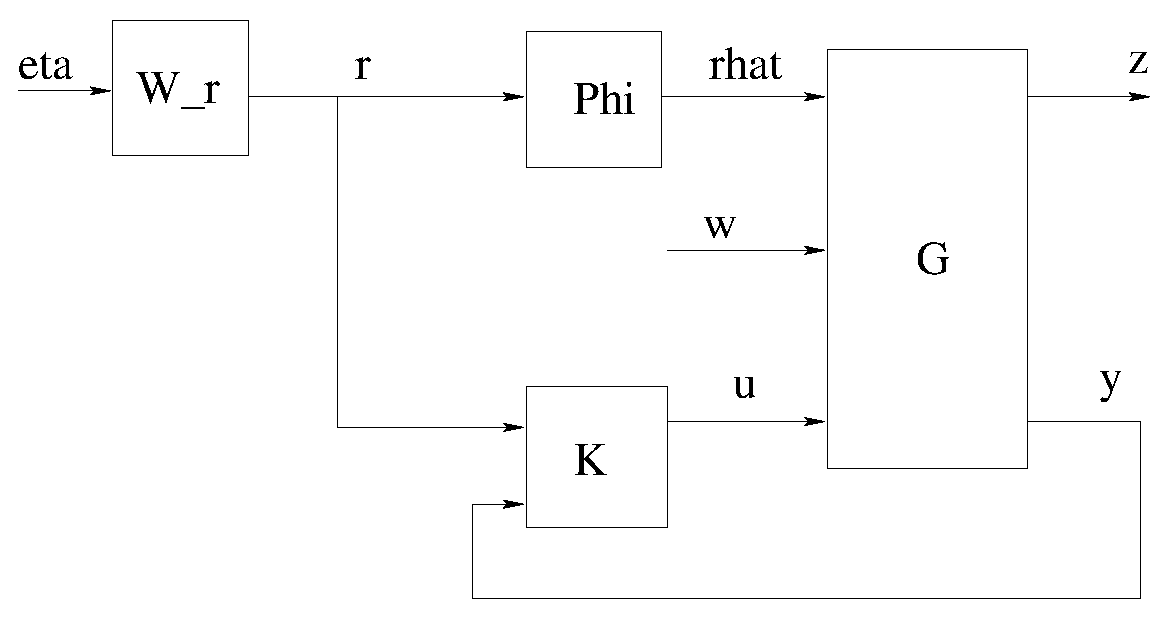
\includegraphics[height=4.0cm]{./diags/DistRejSys.eps}
\caption{\label{fig:DistRejSys} A generalized regulator problem with both previewable and non-previewable disturbances. The transfer function $G$ is the system to be controlled, $K$ is the controller to be synthesized and $\Phi$ is an $N$-step delay line. The disturbance $w$ is not previewable, the control and measurement signals are $u$ and $y$ respectively, $\hat r$ is the previewable disturbance, and $r$ is the future value of $\hat r$. The filter $W_r$ is used  model the expected frequency content of $r$.}
\end{center}
\end{figure}

One of the first papers to recognise the importance of preview control is \cite{Sheridan}, in which three preview control models are described. In the third of these models open-loop optimal preview controls are found using dynamic programming. The earliest applied work on preview control dates back to \cite{Bender_1968_PrevSusp}, where Wiener filter theory was used to design an active suspension with road preview. This solution was not implementable as it required the transfer function from the previewed path to the vehicle's acceleration to be unstable. Much of the subsequent work on preview tracking has its origins in the 1973 PhD thesis of M. Tomizuka~\cite{Tomi_1973_Thesis}, in which  the preview control task is cast in a discrete-time linear quadratic regulator framework by augmenting the plant dynamics with a delay line model. In this formulation the number of states grows in direct proportion to the preview length and so a direct solution of the corresponding Riccati equations becomes computationally infeasible for long preview lengths. Tomizuka presented an efficient recursive method for solving these large equations. A continuous-time version of a LQ preview control problem is studied in \cite{Tomizuka_1975_ContinuousLQPreview}, while a continuous-time preview control problem is given a stochastic interpretation in \cite{Lindquist}.

In the context of the early literature, \cite{Tomizuka_1975_OptDiscretePreview} provides a good overview of an output-feedback preview-tracking problem with reference noise. This paper also summarizes many of the basic properties of preview feedback controllers. 
Motivated by a process control problem, another previewable command reference variant, the so-called proportional, integral, derivative, preview (PIDP) controller is studied in \cite{Tomizuka_1979_IntegralPreviewFI} in an LQ optimal control framework. A closely associated feedforward problem is studied in \cite{Tomi_1980_FFPrev}. Other schemes for computing a feedforward-only controller is given in \cite{Zattoni_2006_H2PreviewFF} and \cite{Marro_2005_FFH2Preview}. Bender's vehicle suspension preview problem is re-visited in \cite{Tomi_1976_SuspRevisited} in a discrete-time command preview framework. The preview suspension problem has attracted the attention of several practitioners in the more recent literature; examples include \cite{Hac_1992_Opt_Veh_Susp,Marzbanrad_2004_SuspPrev,Roh_1999_Stoc_Opt_Prev,Sharp_2005_CarHandlingPreview}.

We will use the problem formulation in Figure \ref{fig:DistRejSys} as a basis for the results presented here. A solution will be derived
by formulating the problem in a generalised regulator framework \cite{LimebeerGreen,ZDG}, and then finding efficient solutions to the resulting high-dimension Riccati equations. Contributions made by this paper include:
\begin{itemize}
\item An efficient method for finding the $\htwo$ norm of the closed-loop system;
\item a method for evaluating the benefit of preview;
\item a low-order output feedback controller implementation;
\item an analysis of the  generic properties of preview controllers.
\end{itemize}

Figure~\ref{fig:SimpleSISOPrev} illustrates a simple example that may be used to highlight the benefit of preview, the broad structure of the controller, and the effect of preview on the achievable $\htwo$-norm of the closed-loop system. In this formulation, the preview action arises because of the delay line $\Phi$. The input to the controller is $r$, which is the future value of the reference, and $K$ is chosen so as to ensure that $e$ is `small', and hence the plant output follows $\Phi r$ as closely as possible. 
\begin{figure}
\stdcontrolfrags
\begin{center}
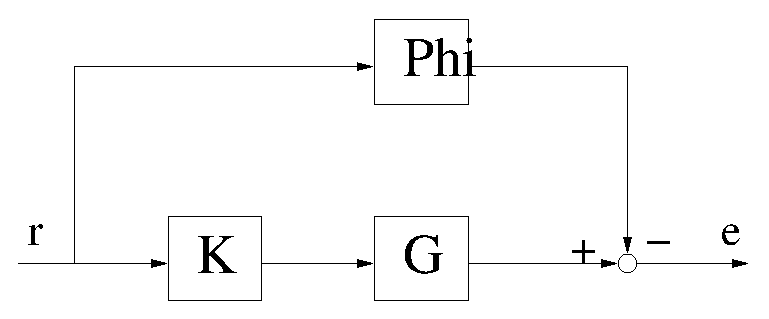
\includegraphics[width=0.4\hsize]{./diags/SimpleExampleNominalNoK2.eps}
\end{center}
\caption{A simple SISO open-loop preview tracking problem. The transfer function $\Phi=\z^{-N}$ is an $N$-step delay, $G$ is the plant to be controlled, and $K$ is a feedforward controller. The signal $r$ is the \textit{future} value of the reference, and $e$ is the tracking error.}
\label{fig:SimpleSISOPrev}
\end{figure}
%
Now define the error system:
\als{E(\z)=G(\z)K(\z)-\Phi(\z),}
and assume that $G(\z)$ is stable; in the case that $G(\z)$ is unstable, it could be replaced by $\hat G(\z)=G(\z)(1-G(\z)K_f(\z))^{-1}$ in which $K_f(\z)$ is a stabilising feedback controller. Providing that $G(\z)$ has all its zeros inside the unit circle, perfect tracking ($E(\z)=0$) may be achieved by simply setting $K(\z)=G(\z)^{-1}\Phi(\z)$. 
However, if $G(\z)$ is {NMP}, then such a $K(\z)$ is not internally stabilising and a controller must be found that recognises the limits imposed by {NMP} zeros on the achievable tracking performance. %Such limitations are well known for non-preview systems (i.e. $N=0$ and $\Phi=1$), and are investigated in some detail in \cite{Middleteon_2004_PrevPerf} and \cite{Mirkin_2004_FixedLagPerfSaturation} for the preview case.

For the case where $G(\z)$ is an arbitrary stable, rational transfer function having a single real {NMP} zero at $c_z$, an algebraic expression for the $\htwo$-optimal controller will now be found. Our objective is to find an internally stabilising $K(\z)$ such that $\nrm{E(\z)}_2$ is minimised. 

The following inner-outer factorization  may be performed:
\als{G(\z)&= G_o(\z) G_i(\z),
\intertext{where: }
G_i(\z)&=\frac{\z-c_z}{1-\z c_z}
.}
We can write $E(\z)= (\tilde{K}(\z) -\Phi(\z)G_i(\z^{-1}))G_i(\z)$ in which $\tilde{K}(\z)= K(\z) G_o(\z)$ and:
\mbox{$G_i(\z^{-1})G_i(\z)=1$}. The optimal controller is found by setting $K(\z) = (\Phi(\z)G_i(\z^{-1}))_+ G_o^{-1}(\z) $, where $(\cdot)_+$ denotes the stable projection \citep{Doyle_1990_FeedbackControlTheory}. 
It follows by direct calculation  that:
\aln{K(\z)&=\underbrace{G_o(\z)^{-1}}_{IIR}\underbrace{\left(-c_z^{-1}\z^{-N} +  (1-c_z^{-2})c_z \sum^N_{i=1}(\z^{i-N}/c_z^i) \right)}_{FIR},\nonumber
\intertext{and that:}
\nrm{E(\z)}_2&=\frac{1}{\left|c_z^{N+1}\right|}\sqrt{c_z^2-1}.\label{eqn:H2normsimple}}
%


 
Since $\nrm{E(\z)}_2\rightarrow 0$  as $N\rightarrow \infty$, we conclude that in this example preview action can overcome completely the tracking limitation
imposed by the {NMP} zero. The optimal controller contains a high-order {FIR} part and a low-order {IIR} part, where the preview action comes from the {FIR} part. The dynamics of the {FIR} block is  fully specified by the {RHP} zero, $c_z$, and the preview length, $N$. The fact that the high order part of the controller is FIR leads to an efficient hardware implementation.
%A similar structure is also observed in the solution to the synthesis problem of Figure~\ref{fig:DistRejSys}, and leads to an efficient implementation of the high-order controller. 

A pole-zero plot of the optimal controller is given in Figure \ref{fig:PZforSISOPrevH2} for the case where $c_z=1.05$, $G_o(\z)=(1-\z c_z)/(\z-0.5)$, and $N=20$. Notice the almost pole-zero cancellation on the real axis. In the limit $N\rightarrow \infty$ cancellation occurs. 
\begin{figure}
\begin{center}
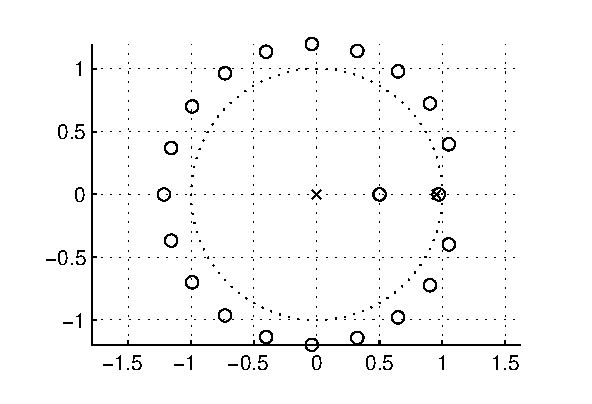
\includegraphics[width=8cm]{./diags/SimpleExamplePZPlot2.eps}
\end{center}
\caption{Pole-zero plot of the $\htwo$-optimal $K(\z)$ for the case where $c_z=1.05$, $G_o(\z)=(1-\z c_z)/(z-0.5)$ and $N=20$.   }
\label{fig:PZforSISOPrevH2}
\end{figure}
This simple preview problem highlights several important features that will be carried over into the more complex problem treated in this paper. In particular:
\begin{enumerate}
\item The preview action is captured in an {FIR} block having order $N$.
\item The remainder of the controller (the {IIR} part) has order equal to the plant order.
\item The preview length (N) required to achieve 95\% (for example) of the maximum norm reduction due to preview, is affected by the position of {NMP} zeros. 
\end{enumerate} 

Point 3 merits further discussion. A central tenet of this paper is that the preview length could be sufficiently large that solution of the associated {DARE} is computationally intractable. However, it might be argued that it is never necessary to use a large preview length because one could simply reduce the sampling rate until $N$ becomes sufficiently small.  In \cite{Middleteon_2004_PrevPerf}, an example similar to Figure \ref{fig:SimpleSISOPrev} is treated in continuous-time, and it is found that the required preview \textit{time} is purely a function of the position of the continuous-time zero. The discrete-time equivalent of this result is: for a given performance improvement, the preview time $NT_s$ (where $T_s$ represents the sample time) is determined by the position of the continuous-time zero. This fact can be seen by considering the effect of $T_s$ on the magnitude of $c_z$ in (\ref{eqn:H2normsimple}). Typically, the sampling rate is determined by the frequency at which tracking or disturbance rejection is required, and also by the frequency of any unstable poles \citep{Houpis_1991_DigitalControlSystems}. It therefore follows that a combination of low frequency zeros (which impose a large $NT_s$), and higher frequency performance specifications or unstable poles (which impose a low $T_s$), would lead unavoidably to a large preview length ($N$).% in order to achieve 95\% of the maximum available benefit due to preview.

%An obvious conclusion to be drawn from the example in this section is that preview is potentially useful when designing feedforward controllers for {NMP} systems. However, if one has a control problem with an unstable plant, which is stabilised by a feedback controller, then the resulting closed-loop will often be {NMP}, and so preview action is also potentially useful when controlling unstable systems.

At this stage, the reader might be left with the impression that preview is of no benefit for {MP} plants. However, as an example, it can be shown that the minimum achievable $\htwo$-norm of the transfer function:
\als{
\ma{E(\z)\\\rho K(\z)}
,}
is reduced by preview action, even when $G(\z)$ is {MP}. By adding the additional term $\rho K(\z)$ into the optimisation,
we are effectively penalising the magnitude of the control action. In general, a large $\rho$ leads to a slow response and so a large $N$ is required in order to get the full benefit from preview action. A detailed analysis of the effects of preview on systems of this form is given in \cite[Chapter 4]{Hazell_2007_Thesis}

The paper is structured as follows: Preliminaries and some standard notation is given in Section~\ref{sec:notation}. A state-space description of the generalized regulator problem with both previewable and non-previewed exogenous disturbances is derived in Section~\ref{sec:Sys}. The solution of this problem, which is illustrated in Figure~\ref{fig:DistRejSys}, is the central focus of the paper. Following a summary of the general theory, the full-information preview control problem is solved in Section~\ref{sec:H2FI}. The results are mainly concerned with efficient algorithms for solving the $\htwo$ full-information Riccati equation, and the evaluation of the full-information feedback gain matrix. The solution of the output feedback preview problem is given in Section~\ref{sec:H2OF}. The output feedback controller involves a combination of a state-estimator, and the solution to the full-information problem. An efficient controller synthesis is also given in this section. The effect of preview in reducing the $\htwo$-norm of the closed-loop system is analysed in Section~\ref{sec:2norm}. The special case of feedforward control with preview is analysed in Section~\ref{sec:Preproc}. A summary of the main features of preview controllers, as well as some design insights, are given in Section~\ref{sec:H2PrevSum}. The conclusions are given in Section~\ref{sec:Conclusions}.
 
\section{Notation and Preliminaries}
\label{sec:notation}
We will make use of discrete-time state-space models of the form:
\als{
x(k+1)&=Ax(k)+Bu(k)\\
y(k)&=Cx(k)+Du(k)
}
in which $k$ is the time index, $x(k)$ is a vector of state variables, $u(k)$ is a vector of inputs, $y(k)$ is a vector of outputs, and $A,B,C$ and $D$ are appropriately dimensioned real matrices. Signals will sometimes be represented by omitting the time index, e.g.
$$x=\{x(k)\}^{\infty}_{-\infty}.$$
When transfer functions are associated with these models, they are computed using:
\als{
G(\mathcal{Z})=C(\mathcal{Z} I -A)^{-1}B+D
}
in which $\mathcal{Z}$ is the Z-transform variable. We will also use the shorthand notation:
\aln{
G(\mathcal{Z})\shorteq\ssmodf{A}{B}{C}{D}\label{eqn:GABCD}.
}
The transfer function $G(\mathcal{Z})$ will be abbreviated by $G$ when no confusion will occur.

The (lower) linear fractional transformation of the transfer-function matrices $P=\ma{P_{11} &P_{12}\\P_{21} & P_{22}}$, and $K$ will be written as $F_l(P,K)$ where: 
 \als{F_l(P,K)=P_{11}+P_{12}K(I-P_{22}K)^{-1}P_{21}.} 

The trace of a matrix will be denoted $\tra{A}$.
 
The $\htwo$-norm of a transfer function $G(\mathcal{Z})$ will be denoted by $\nrm{G(\z)}_2$, and is defined by:
\als{\nrm{G(\z)}_2=\frac{1}{2\pi}\int_{-\pi}^{\pi}\tra{G(e^{j\theta})'G(e^{j\theta})}\textrm{d}\theta.}
If $G$ has the realisation (\ref{eqn:GABCD}), with $A$ assumed stable, and $X$ is a matrix which satisfies:
\aln{
X&=A'XA+C'C, \nonumber\\
\intertext{then}
\nrm{G(\z)}^2_2&=\tra{B'XB+D'D}\label{eqn:2normcomp}
.}
%
A transfer function that maps signal $a$ to signal $b$ will be denoted $T_{a\rightarrow b}$.

% The product operator will have the definition:
% \als{\prod_{i=1}^{N} T_i= T_1T_{2}\ldots T_{N-1} T_N }
%The set of eigenvalues of $A$ will be denoted as $\lambda(A)$ and the eigenvalues of the matrix pencil $A-\lambda B$ will be written as $\lambda(A,B)$. 
An $m\times p$ dimensional zero matrix will be denoted as $0_{m\times p}$ and an $n$ dimensional identity matrix will written as $I_n$. The shorthand $0_m=0_{m\times m}$ will also be used. %We will often use the notation $\star_{m\times p}$ to represent a matrix belonging to $\mathbb R^{m\times p}$; the dimensions may be omitted when no ambiguity will result.

The complex conjugate transpose of $A$ will be denoted $A'$ and n-dimensional real vectors are denoted $\mathbb{R}^n$.


%The largest singular value of $A$ will be denoted as $\bar\sigma(A)$.

 
\section{Problem formulation}
\label{sec:Sys}
The $\htwo$-optimal preview controller is defined to be the $K$ that minimises $\nrm{T_{v\rightarrow z}}_\infty$, where $v=\ma{\eta'&w'}'$ with $w,\eta$ and $z$ defined in Figure \ref{fig:DistRejSys}. In other words, we wish to choose $K$, which minimises $\Vert F_l(P,K) \Vert_2$, where $P$ is the mapping:
\als{
\ma{\arr{c}{z\\\hline y\\r}}=\ma{P_{11} & P_{12}\\P_{21} & P_{22}}\ma{\arr{c}{ \eta\\w \\\hline u}}
.}

The signals satisfy: $\szo{w(k)}{l_w}$, $\szo{r(k)}{l_r}$, $\szo{\eta(k)}{l_r}$, $\szo{v(k)}{l}$ (i.e. $l=l_r+l_w$), $\szo{u(k)}{m}$, $\szo{y(k)}{q_g}$   and $\szo{z(k)}{p}$.  Also define $q=q_g+l_r$. The  $N$-step delay line, $\Phi$, has the realisation:

\[
\Phi(\z)=\z^{-N}I_{l_r} \shorteq \ma{\arr{c|c}{A_p&B_p\\\hline C_p&0_{l_r\times l_r}}}
\]
with $A_p,B_p$ and $C_p$ defined by:
 \als{
 A_p&=\ma{  0_{l_r}&I_{l_r} &\hdots&  0_{l_r}\\
   \vdots&\vdots &&  \vdots\\
   0_{l_r}&0_{l_r} &\hdots&  I_{l_r}\\
   0_{l_r}&0_{l_r} &\hdots&  0_{l_r}}
 %A_p&=\ma{0&I_{(N-k-1)lr}\\0_{l_r\times l_r}&0}
 \intertext{and}
 B_{p}&=\ma{0_{(N-1)l_r\times l_r} \\ I_{l_r}},  \quad  
 C_p=\ma{\arr{c}{\arr{cccc}
 {I_{l_r}& 0_{l_r\times (N-1)lr}}
 }}
}
where $N$ represents the number of preview steps and $\szo{A_p}{Nl_r\times Nl_r}$.
 Without loss of generality the square transfer function $W_r$ is assumed to be outer \cite{LimebeerGreen,ZDG}, with realisation:
\als{
W_r\shorteq \ma{\arr{c|c}{
A_r & B_r\\ \hline
C_r & D_r
}}
}
where $\szo{A_r}{n_r\times n_r}$. Also without loss of generality \cite{LimebeerGreen}, the plant is assumed to have the realisation:

\als{
G\shorteq \ma{\arr{c|cc:c}{
A_g & B_{1gr} & B_{1gw} & B_{2g}\\\hline
C_{1g}& D_{11gr} & D_{11gw} & D_{12}\\\hdashline
C_{2g}&D_{21gr} & D_{21gw}&0
}}
}
where $\szo{A_g}{n_g\times n_g}$. 

The transfer function from $\eta$ to $\ma{\hat r\\r} $ has realisation:

\als{
\ma{\arr{c|c}{
A_d&B_d\\\hline
C_{d1}&0\\\hdashline
C_{d2}&D_r
}}
=\ma{\arr{cc|c}{
A_p &B_pC_r&B_pDr\\
0&A_r&B_r\\\hline
C_p&0&0\\\hdashline
0&C_r&D_r
}},
}
and so the generalised plant $P$ has realisation:
\aln{
P&\shorteq
\arr{c}{
\hspace{1.5cm}\stackrel{n_g}{\leftrightarrow}\hspace{0.5cm}
\stackrel{Nl_r+n_r}{\leftrightarrow}\hspace{0.9cm}
\stackrel{l_r}{\leftrightarrow}\hspace{0.6cm}
\stackrel{l_w}{\leftrightarrow}\hspace{0.8cm}
\stackrel{m}{\leftrightarrow} \\
%%
\arr{r}{
\scriptstyle{n_g} \,\updownarrow\\
\scriptstyle{Nl_r+n_r} \,\updownarrow\\
\scriptstyle{p} \,\updownarrow\\
\scriptstyle{q} \,\updownarrow\\
\scriptstyle{l_r} \,\updownarrow} 
\ma{\arr{cc|cc:c}{
A_g&B_{1gr}C_{d1}&0&B_{1gw}&B_{2g}\\
0&A_d&B_{d}&0&0\\\hline
C_{1g} &D_{11gr}C_{d1} &0&D_{11gw}&D_{12}\\ \hdashline
C_{2g}&D_{21gr}C_{d1}&0&D_{21gw}&0\\
0&C_{d2}&D_r&0&0
}}}\label{eqn:P}\\
&\shorteq\ssmod{A}{B_1}{B_2}{C_1}{C_2}{D_{11}}{D_{12}}{D_{21}}{0}. \label{eqn:GenPlant}
}
The $A$-matrix in (\ref{eqn:GenPlant}) satisfies $\szo{A}{n\times n}$ with $n=n_g+Nl_r+n_r$.





 
\section{Full-information control problem}
\label{sec:H2FI}
%\label{subsec:StandardFI}
\subsection{Standard Theory}
\label{subsec:stdH2FI}
We begin with a brief summary of the discrete-time, linear time-invariant perfect information control problem \cite{LimebeerGreen}, which has plant description
$$P_{FI} \shorteq \arr{c}{\hspace{0.8cm}\stackrel{n}{\leftrightarrow}\hspace{0.5cm}\stackrel{l}{\leftrightarrow}\hspace{0.6cm}\stackrel{m}{\leftrightarrow} \\\arr{r}{\scriptstyle{n} \,\updownarrow\\\scriptstyle{p} \,\updownarrow\\\scriptstyle{n} \,\updownarrow\\\scriptstyle{l} \,\updownarrow} \ma{\arr{c|cc}{ A&B_1&B_2\\\hline C_1&D_{11}&D_{12}\\I&0&0\\0&I&0}}},$$and which satisfies the following standard assumptions:
\begin{itemize}
\item[(A1)] $(A,B_2)$ is stabilisable 
\item[(A2)] $D_{12}'D_{12}>0$
\item[(A3)] rank$\ma{A-e^{j\theta}I&B_2\\C_1& D_{12}}=n+m \quad \forall\, \theta \,\in (-\pi,\pi]$.
\end{itemize}

We would like to find the internally stabilising controller $K_{FI}$ which minimises $\nrm{F_l(P_{FI},K_{FI})}_2$. First define:
\aln{
\bar R&=D_{12}'D_{12}+B_2'XB_2   \\
  F_2&=-{\bar R}^{-1}(B_2'XA+D_{12}'C_1)  \label{eqn:F2Def}\\
A_c&=A+B_2F_2.
}

In \cite{ZDG} it is shown that if (A1)-(A3) are satisfied then there exists a solution $X$ to the Discrete Algebraic Riccati Equation (DARE):

\aln{X=A'XA-F_2'{\bar R}F_2+C_1'C_1 \label{eqn:X2d}}
such that:
\aln{
&X\geq 0 \label{eqn:Xpos}\\
&A_c \,\, \textrm{is asymptotically stable} \label{eqn:Xstab}
.}

A matrix $X$ satisfying (\ref{eqn:X2d}) and (\ref{eqn:Xstab}) is said to be \textit{stabilising}.

The internally stabilising, full information $\htwo$-optimal controller is then given by:
\begin{equation}
K_{FI}=\ma{F_2 &F_0} \label{eqn:FIcont}
\end{equation} 
with
\[
F_0=-{\bar R}^{-1}(B_2'XB_1+D_{12}'D_{11}).
\]
%
The resulting closed-loop norm is given by:
\mls{
\nrm{F_l(P_{FI},K_{FI})}_2^2= \tra{(D_{11}+D_{12}F_0)'(D_{11}+D_{12}F_0) +(B_1+B_2F_0)'X(B_1+B_2F_0) }.
}


\subsection{Efficient computation of the Full-Information controller}
\label{subsec:FIEff}

In this section we will find an efficient solution for the DARE (\ref{eqn:X2d}) for the plant described in Section \ref{sec:Sys}. First we decompose (\ref{eqn:X2d}) into an $n_g$-dimensional DARE, an $Nl_r+n_r$-dimensional discrete Lyapunov equation, and an $(n_g\times Nl_r+n_r)$-dimensional Stein equation. We then give an efficient solution to the Stein equation, and show how this leads to an efficient method for computing the full information controller.

\begin{lem}[Decomposition of DARE]
Let $X$ be the unique stabilising and nonnegative solution to the DARE (\ref{eqn:X2d}), and partition $X$ as:
%
\als{X&=
	\arr{r}{
	\stackrel{n_g}{\leftrightarrow}\hspace{0.3cm}
	\stackrel{Nl_r+n_r}{\leftrightarrow}\hspace{0.3cm}\\
	%%
	\arr{r}{
	\scriptstyle{n_g} \,\updownarrow\\
	\scriptstyle{Nl_r+n_r} \,\updownarrow}
	\ma{\arr{cc}{ X_{gg} & X_{gd} \\ X_{gd}' & X_{dd}}}
,}}
%
then $X_{gg}$ is the unique stabilising and nonnegative solution to the DARE:
\aln{X_{gg}&=A_g'X_{gg}A_g - F_{2g}'{\bar R}F_{2g}+C_{1g}'C_{1g}, \label{eqn:Xgg}
\intertext{where}
F_{2g}&=-\bar R^{-1}\left(B_{2g}'X_{gg}A_g+D_{12}'C_{1g}\right) \label{eqn:F2g}\\
\intertext{in which $\bar R$ may be computed from}
\bar R&=B_{2g}'X_{gg}B_{2g}+D_{12}'D_{12}\label{eqn:RbEff}.
\intertext{Further, $X_{gd}$ and $X_{dd}$ are the unique solutions to}
X_{gd}&=SC_{d1}+A_{cg}'X_{gd}A_d  \label{eqn:Xgd}\\
X_{dd}&=A_d'X_{dd}A_d+Q  \label{eqn:Xdd},}
with
\als{
S&=A_g'X_{gg}B_{1gr}+F_{2g}'B_{2g}'X_{gg}B_{1gr}+F_{2g}'D_{12}'D_{11gr}+C_{1g}'D_{11gr}\\
A_{cg}&=A_g+B_{2g}F_{2g}\\
F_{2d}&=-\bar R^{-1}\left( B_{2g}'X_{gd}A_d+B_{2g}'X_{gg}B_{1gr}C_{d1}+D_{12}'D_{11gr}C_{d1} \right)\\
Q&=C_{d1}'B_{1gr}'X_{gg}B_{1gr}C_{d1}+A_d'X_{gd}'B_{1gr}C_{d1}+C_{d1}'B_{1gr}'X_{gd}A_d\\
&\qquad-F_{2d}'\bar RF_{2d}+C_{d1}'D_{11gr}'D_{11gr}C_{d1}.
}
\end{lem}

\begin{proof}
First partition (\ref{eqn:F2Def}) conformably with $X$:
\aln{
F_2&=-\bar R^{-1}\left( \ma{B_{2g}' & 0 } \ma{X_{gg} & X_{gd} \\ X_{gd}' & X_{dd}}\ma{A_g & B_{1gr}C_{d1}\\ 0 & A_d}+D_{12}'\ma{C_{1g} & D_{11gr}C_{d1}}\right) \nonumber \\
&=-\bar R^{-1}\ma{B_{2g}'X_{gg}A_g+D_{12}'C_{1g} & B_{2g}'X_{gd}A_d+B_{2g}'X_{gg}B_{1gr}C_{d1}+D_{12}'D_{11gr}C_{d1}} \nonumber \\
&=\ma{F_{2g} &F_{2d}}\label{eqn:F2part}
,}
and hence $F_{2g}$ and $F_{2d}$ form partitions of $F_2$.
Now partition (\ref{eqn:X2d}) to obtain:

\mln{
\ma{X_{gg} & X_{gd} \\ X_{gd}' & X_{dd}}=\ma{A_g' &0 \\ C_{d1}'B_{1gr}' & A_d'}\ma{X_{gg} & X_{gd} \\ X_{gd}' & X_{dd}} \ma{A_g & B_{1gr}C_{d1}\\ 0 & A_d}\\
	-\ma{F_{2g}'\\F_{2d}'}\bar R\ma{F_{2g}&F_{2d}}+\ma{C_{1g}'\\C_{d1}'D_{11gr}'}\ma{C_{1g}&D_{11gr}C_{d1}}.
	\label{eqn:RicXpart}
}
Equation (\ref{eqn:RbEff}) is easily checked, and so equations (\ref{eqn:Xgg}), (\ref{eqn:Xgd}) and (\ref{eqn:Xdd}) follow immediately by considering, respectively, the top left, the top right, and the bottom right partitions of (\ref{eqn:RicXpart}).

Now note that:
\als{
A_c=\ma{A_{cg} & \star \\ 0 & A_d}
}
in which $A_d$ is stable.  It now follows from assumption (A1) that $X_{gg}$ is stabilising if and only if $X$ is stabilising.
\end{proof}
%

Note that $F_{2g}$ and $\bar R$ are not functions of $X_{gd}$ or $X_{dd}$, and so (\ref{eqn:Xgg}) may be solved independently of (\ref{eqn:Xgd}) and (\ref{eqn:Xdd}). Since (\ref{eqn:Xgd}) depends on the solution of (\ref{eqn:Xgg}), it can be solved next. Finally (\ref{eqn:Xdd}) depends on both (\ref{eqn:Xgg}) and (\ref{eqn:Xgd}) and so is necessarily solved last. The following result provides a fast algorithm for solving (\ref{eqn:Xgd}).

\begin{lem}[Efficient solution of Stein equation]
\label{lem:SylvRecurs}
Consider the discrete Stein equation:
\aln{
X_{gd}=SC_{d1}+A_{cg}'X_{gd}A_d \label{eqn:SylvX}
}
with $A_{cg}$ stable. Partitioning   $X_{gd}=\ma{X_{gp} & X_{gr}}$ compatibly with  
\als{A_d=\ma{A_p & B_pC_r\\0& A_r},}
gives
\aln{
X_{gp}&= \ma{S &A_{cg}'S & {A_{cg}'}^2S & \ldots&{A_{cg}'}^{N-1}S }\label{eqn:Xgp}\\ 
X_{gr}&={A_{cg}'}^{N}SC_r+A_{cg}'X_{gr}A_r \label{eqn:Xgr}.
}

\begin{proof}
Partitioning (\ref{eqn:SylvX}) leads to :
\aln{
X_{gp}&=SC_p+A_{cg}'X_{gp}A_p  \label{eqn:XgpSyl}\\
X_{gr}&=A_{cg}'X_{gp}B_pC_r+A_{cg}'X_{gr}A_r.  \label{eqn:XgrSyl}
}
%
If we substitute (\ref{eqn:XgpSyl}) into itself $M$ times we obtain:
\als{
X_{gp}&=  {A_{cg}'}^{M+1} X_{gp} A_p^{M+1}+\sum_{k=0}^{M} {A_{cg}'}^k SC_p A_p^k.
}
Since $A_{cg}$ and $A_p$ are stable, we may allow $M\rightarrow \infty$  and hence write:
\als{
X_{gp}&= \sum_{k=0}^{\infty} {A_{cg}'}^k SC_p A_p^k.
}
However, since $A_p^N=0$ we may truncate the infinite sum to give:
\aln{
X_{gp}&= \sum_{k=0}^{N-1} {A_{cg}'}^k SC_p A_p^k.\label{eqn:XgpSum}
}
The effect of postmultiplying by $A_p^k$ is to shift the columns of the preceding matrix right by $kl_r$, and so $C_pA_p^k=\ma{0_{l_r\times kl_r} &I_{l_r}&0_{l_r\times (N-1-k)l_r }}$. Substituting this into (\ref{eqn:XgpSum}) leads to (\ref{eqn:Xgp}). Now substituting (\ref{eqn:Xgp}) into (\ref{eqn:XgrSyl}) leads to (\ref{eqn:Xgr}).
\end{proof}
\end{lem}

The following is obtained by substituting (\ref{eqn:Xgp}) and (\ref{eqn:Xgr}) into the definitions for the controller gains $F_2$ and $F_0$.

\begin{cor}[Efficient computation of Full-Information controller gains]
The matrix $F_2$ may be partitioned (compatibly with $A$) as $F_2=\ma{F_{2g}&F_{2p}&F_{2r}}$ in which $F_{2g}$ is given by (\ref{eqn:F2g}), and 
\aln{
F_{2p}&=-{\bar R}^{-1}\ma{B_{2g}'X_{gg}B_{1gr}+D_{12}'D_{11gr} & B_{2g}'S & B_{2g}'A_{cg}'S& \ldots & B_{2g}'{A_{cg}'}^{N-2}S}\label{eqn:F2pEff}\\
F_{2r}&=-{\bar R}^{-1}\left(  B_{2g}'{A_{cg}'}^{N-1}SC_r+B_{2g}'X_{gr}A_r \right)\label{eqn:F2rEff}
.}
If we partition $F_0=\ma{F_{0r}& F_{0w}}$ then:
\aln{
F_{0r}=-{\bar R}^{-1}\left(  B_{2g}'X_{gr}B_r+B_{2g}'A_{cg}^{N-1}SD_r \right)\label{eqn:F0reff}\\
F_{0w}=-{\bar R}^{-1}\left(  B_{2g}'X_{gg}B_{1gw}+D_{12}'D_{11gw} \right)\label{eqn:F0w}
.}
\end{cor}


\begin{cor}
As $N\rightarrow \infty$ the control becomes independent of the choice of $W_r$
\end{cor}
\begin{pf}
Since $A_r$ and $A_{cg}$ are asymptotically stable, it follows from standard results that (\ref{eqn:Xgr}) has a unique solution. In the limit as $N\rightarrow\infty$, (\ref{eqn:Xgr}) implies that $X_{gr}=A_{cg}'X_{gr}A_r$ and so in the limit $X_{gr}=0$. Direct substitution into (\ref{eqn:F2rEff}) and (\ref{eqn:F0reff}), while taking the limit as $N\rightarrow \infty$, leads to
\als{
F_{2r}=0 \text{ and }  F_{0r}=0 \quad \forall A_r,B_r,C_r,D_r
,}
and so the control signal is independent of $W_r$.
\end{pf}

\begin{rem}
\label{rem:PrevGainInterp}
If $x_g$ and $x_r$ are the states of $G$ and $W_r$ respectively, then the optimal control is given by:
\als{
u(k)^*&=\underbrace{F_{2g}x_g(k)}_{\mbox{feedback}}+\underbrace{F_{2r}x_r(k)+F_{0r}\eta(k)+F_{0w}w(k)+\sum_{j=0}^{N-1}{F_{2p,j}r(k-N+j)}}_{\mbox{feedforward}}
\intertext{with}
F_{2p,0}&=-{\bar R}^{-1}\left(B_{2g}' X_{gg}B_{1gr}+D_{12}'D_{11gr}\right)\\
F_{2p,j}&=-{\bar R}^{-1}B_{2g}' A_{cg}^{j-1}S \quad 1\leq j\leq N-1.
}
\end{rem}

\begin{rem}
\label{rem:SmallPrevGain}
The feedback gain, $F_{2g}$, is precisely that which would be obtained if one were to search for a full information controller that minimised $\nrm{T_{w\rightarrow z}}$, with $W_r$ and $\Phi$ removed from the problem description. The choice of feedback control is therefore independent of the preview length.
\end{rem}

\begin{rem}
\label{rem:FIminwandr}
The full-information controller which minimises $\nrm{T_{v\rightarrow z}}_2$ also minimises $\nrm{T_{\eta\rightarrow z}}_2$ and $\nrm{T_{w\rightarrow z}}_2$. This type of relationship is true for any partition of the exogenous disturbance signal in an $\htwo$ full-information generalised regulator problem, and it is not a particular feature of the preview control problem. To see this, note that the two minimisation problems:
\begin{eqnarray}
\min_{K_{FI}}\nrm{T_{\eta\rightarrow z}}_2 \label{norm1} \\
\min_{K_{FI}}\nrm{T_{w\rightarrow z}}_2, \label{norm2}
\end{eqnarray}
are related by the choice of $B_1$ and $D_{11}$, and that computation of the controller gain $F_{2}$ is independent of these matrices. The feedforward control gains $F_{0r}$ and $F_{0w}$ can be chosen independently, and so it is possible to simultaneously minimise $\nrm{T_{\eta\rightarrow z}}_2$ and $\nrm{T_{w\rightarrow z}}_2$. Since $\nrm{T_{v \rightarrow z}}^2_2 = \nrm{T_{\eta\rightarrow z}}^2_2 + \nrm{T_{w \rightarrow z}}^2_2$, a controller satisfying (\ref{norm1}) and (\ref{norm2}) also minimizes $\nrm{T_{v \rightarrow z}}_2$.
\end{rem}



\section{Output feedback solution}
\label{sec:H2OF}
\subsection{Standard Theory}
\label{subsec:stdH2OF}
We now consider a discrete-time, linear, time-invariant system, $P$, of the form $$P \shorteq \arr{c}{\hspace{0.8cm}\stackrel{n}{\leftrightarrow}\hspace{0.5cm}\stackrel{l}{\leftrightarrow}\hspace{0.6cm}\stackrel{m}{\leftrightarrow} \\\arr{c}{\scriptstyle{n} \,\updownarrow\\\scriptstyle{p} \,\updownarrow\\\scriptstyle{q} \,\updownarrow} \ma{\arr{c|cc}{ A&B_1&B_2\\\hline C_1&D_{11}&D_{12}\\C_2&D_{21}&0}}},$$
which satisfies (A1)-(A3) as well as:
\begin{itemize}
\item[(A4)] $(A,C_2)$ is detectable 
\item[(A5)] $D_{21}D_{21}'>0$
\item[(A6)] rank$\ma{A-e^{j\theta}I&B_1\\C_2& D_{21}}=n+q\quad \forall\, \theta \,\in (-\pi,\pi]$.
\end{itemize}
%
We wish to compute an internally stabilising $K$ that minimises $\nrm{F_l(P,K)}_2$. Define:
\als{
    \bar S&=D_{21}D_{21}'+C_2YC_2' &  L_2&=-(AYC_2'+B_1D_{21}')\bar S^{-1}
}
%
If $(A4)$-$(A6)$ are satisfied, it is shown in \cite{ZDG} that there exists a $Y$ that solves
\aln{
Y=AYA'-L_2 {\bar S}L_2'+B_1B_1'
\label{eqn:Y2d}
}
such that 
\als{
Y\geq 0\\
A+L_2C_2 &\textrm{ is asymptotically stable}.
}
If we define: 
\als{
L_0=(F_2YC_2'+F_0D_{21}'){\bar S}^{-1},
}
then, according to \cite{ZDG}, the $\htwo$-optimal output feedback controller is given by:
\aln{
K& \shorteq \ma{\arr{c|c}{A_K&B_K\\ \hline C_K &D_K}} \label{eqn:H2OptK}\\ 
A_K&=A+B_2F_2+L_2C_2-B_2L_0C_2\\
B_K&=-(L_2-B_2L_0)\\
C_K&=F_2-L_0C_2\\
D_K&=L_0.}

The $\htwo$-norm of the resulting closed loop system is given by:
\mls{\nrm{F_l(P,K)}_2^2=\nrm{F_l(P_{FI},K_{FI})}_2^2\\
	+\tra{\bar R\right( (L_0D_{21}-F_0)(L_0D_{21}-F_0)' +(L_0C_2-F_2)Y(L_0C_2-F_2)'\left) }}


\subsection{Efficient computation of Output Feedback controller}
In this section we aim to find a computationally efficient solution to the DARE (\ref{eqn:Y2d}), given that P has the structure described in (\ref{eqn:P}). The results of this section do not depend on the internal structure of $A_p$, $B_p$ and $C_p$ (though we do require that $A_p$ is stable).

\begin{lem} 
The stabilising non-negative solution to (\ref{eqn:Y2d}) may be computed using:
\als{
Y&=
	\arr{r}{
	\stackrel{n_g}{\leftrightarrow}\hspace{0.2cm}
	\stackrel{Nl_r+n_r}{\leftrightarrow}\hspace{0cm}\\
	%%
	\arr{r}{
	\scriptstyle{n_g} \,\updownarrow\\
	\scriptstyle{Nl_r+n_r} \,\updownarrow}
	\ma{\arr{cc}{ Y_{g} & \hspace{0.2cm}0 \\ 0&\hspace{0.2cm}0}}
	}
,}
where $Y_g$ is the unique stabilising and non-negative solution to:
\aln{
Y_g&=A_gY_gA_g'-L_{2g} {\bar S_g}L_{2g}'+B_{1gw}'B_{1gw} \label{eqn:Y2g}}
with
\als{
\bar S_g&=D_{21gw}D_{21gw}'+C_{2g}Y_gC_{2g}' &  
	L_{2g}&=-(A_gY_gC_{2g}'+B_{1gw}D_{21gw}')\bar S_g^{-1}\nonumber.
}
\end{lem}
\begin{pf}
Note that $(A4)-(A6)$ imply 
\begin{itemize}
\item[(A4g)] $(A_g,C_{2g})$ is detectable; 
\item[(A5g)] $D_{21gw}D_{21gw}'>0$;
\item[(A6g)] rank$\ma{A_g-e^{j\theta}I&B_{1gw}\\C_{2g}& D_{21gw}}=n_g+q_g\quad \forall\, \theta \,\in (-\pi,\pi]$.
\end{itemize}
%
It then follows that $(A4)-(A6)$ ensure the existence of a stabilising nonnegative solution to (\ref{eqn:Y2g}). 
Let $Y_g$ be a stabilising and non-negative solution to (\ref{eqn:Y2g}). We will now show that $Y=\ma{Y_g&0\\0&0}$ is a stabilising nonnegative solution to (\ref{eqn:Y2d}).

It easily checked that the following hold if $Y=\ma{Y_g&0\\0&0}$:
\aln{
\bar S&=\ma{\bar S_g & 0\\0& D_rD_r'}\nonumber\\
L_2&=\ma{L_{2g} &0\\0& -B_dD_r^{-1}}\label{eqn:L2struct}\\
B_1B_1'&=\ma{ B_{1gw}B_{1gw}' & 0\\0& B_dB_d'}\nonumber\\
AYA'&= \ma{A_gY_gA_g'  &0 \\0 &0}\nonumber
,}
where the invertibility of $D_r$ is guaranteed by assumption $(A5)$, together with the fact that $W_r$ is square. It then follows that:
\als{
\spl{AYA'-L_2 {\bar S}\bar L_2'+B_1B_1'&=\ma{A_gY_gA_g'-L_{2g} {\bar S_g}\bar L_{2g}'+B_{1gw}B_{1gw}'&0\\0&0}}\\
&=\ma{Y_g&0\\0&0}=Y.
}
Therefore, if $Y_g$ solves (\ref{eqn:Y2g}), then $Y=\ma{Y_g&0\\0&0}$ solves (\ref{eqn:Y2d}). We now need to check that $Y$ is stabilising. Note that:
\als{
&A+L_2C_2=\ma{A_g+L_{2g}C_{2g}&\star\\0&A_d-B_dD_r^{-1}C_{d2}}.
}
The matrix $A_d-B_dD_r^{-1}C_{d2}$ is stable because:
\aln{
A_d-B_dD_r^{-1}C_{d2}&=\ma{A_p&0\\0&A_r-B_rD_r^{-1}C_r}\label{eqn:AdBdDrCd2},
}
in which $A_p$ is stable by definition and $A_r-B_rD_r^{-1}C_r$ is stable because $W_r$ is assumed to be outer. Since $Y_g$ is stabilising, we know that $A_g+L_{2g}C_{2g}$ is stable, and hence that $A+L_2C_2$ is stable, as required. 
 \end{pf}

\subsection{Efficient implementation}
\label{sec:EffImp}
We now have a complete method for efficiently computing the output feedback preview controller, however, in its present form, this controller has the same order as the generalized plant. In general, a controller of this order cannot be implemented. Fortunately the high-order part of the controller is an FIR filter (illustrated in Figure \ref{fig:PrevContStruct}), for which efficient implementations exist.
{
\stdcontrolfrags
\psfrag{Order ng}{Order $n_g$}
\psfrag{Order nr}{Order $n_r$}
\psfrag{Order Nlr}{Order $Nl_r$}
\psfrag{FIR}{FIR}
\psfrag{IIR}{IIR}
\begin{figure}
\begin{center}
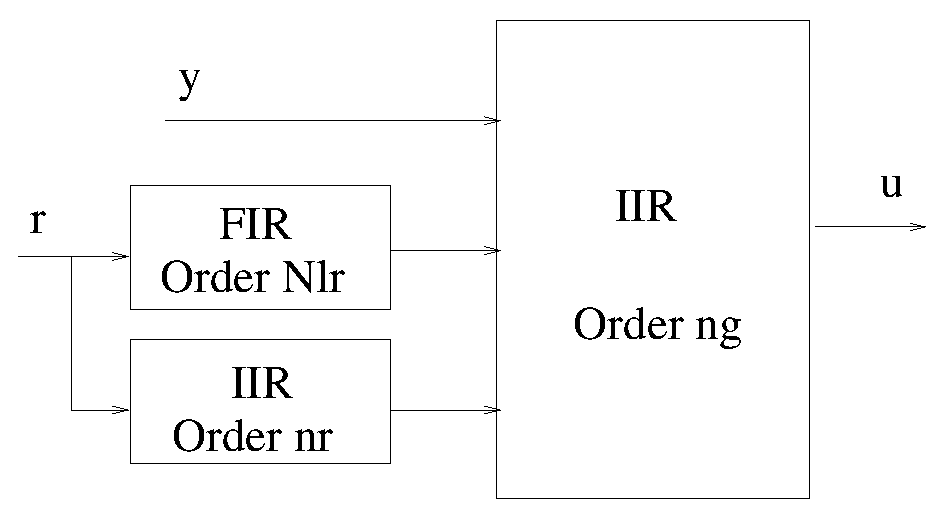
\includegraphics[width=8cm]{./diags/PrevContStruct.eps}
\caption{\label{fig:PrevContStruct} Structure of the $\htwo$-optimal preview controller. The signal $u$ is the control, the measurement is $y$, and $r$ is the future value of the previewable disturbance. The preview length is $N$, $l_r$ is the dimension of $r$, $n_r$ is the order of $W_r$ and $n_g$ is the order of $G$. }
\end{center}
\end{figure}
}


This controller structure is proved in the following Lemma:
%, which just requires the shifting of a block of memory. 


\begin{lem}
The optimal controller described in (\ref{eqn:H2OptK}) for the plant in (\ref{eqn:P}) can be written in the form: 
\aln{
K \shorteq \ma{\arr{c|c}{A_K&B_K\\ \hline C_K &D_K}}
=\ma{\arr{ccc|cc}{A_{Kgg} &A_{Kgp} & A_{Kgr} & B_{Kgy}& B_{Kgr}\\
                  0&A_p&0&0&B_p\\
                  0&0&A_r-B_rD_r^{-1}C_r &0 &B_rD_r^{-1}\\\hline
                  C_{Kg}& C_{Kp}& C_{Kr}& L_{0y}&F_{0r}D_{r}^{-1}}}\label{eqn:StructController}}
where $\szo{A_{Kgg}}{n_g\times n_g}$ and $\szo{B_{Kgg}}{n_g\times l_w}$ and
\als{
L_{0y}&=(F_{2g}Y_gC_{2g}'+F_{0w}D_{21gw}'){\bar S_g}^{-1}\\
A_{Kgg}&=A_g+B_{2g}F_{2g}+L_{2g}C_{2g}-B_{2g}L_{0y}C_{2g} \\
A_{Kgp}&=B_{1gr}C_p+B_{2g}F_{2p}+L_{2g}D_{21gr}C_p-B_{2g}L_{0y}D_{21gr}C_p\\
A_{Kgr}&=B_{2g}F_{2r}-B_{2g}F_{0r}D_r^{-1}C_r\\
B_{Kgy}&=-(L_{2g}-B_{2g}L_{0g})\\
B_{Kgr}&=B_{2g}F_{0r}D_r^{-1}\\
C_{Kg}&=F_{2g}-L_{0y}C_{2g}\\
C_{Kp}&=F_{2p}-L_{0y}D_{21gr}C_p\\
C_{Kr}&=F_{2r}-F_{0r}D_r^{-1}C_r
}
\end{lem}
\begin{pf} The realization given in (\ref{eqn:StructController}) follows from (\ref{eqn:H2OptK}), together with (\ref{eqn:L2struct}),  (\ref{eqn:AdBdDrCd2}) and:
\als{L_0=\ma{L_{0y} & F_{0r}D_r^{-1}}.}
\end{pf}
%
This then leads to the low-order implementation:
\begin{equation}
\bar K \shorteq \ma{\arr{cc|ccc}{A_{Kgg}  & A_{Kgr} & B_{Kgy}& A_{Kgp} &B_{Kgr}\\
                  0&A_r-B_rD_r^{-1}C_r &0 &0&B_rD_r^{-1}\\\hline
                  C_{Kg}&  C_{Kr}& L_{0y}&C_{Kp}&F_{0r}D_{r}^{-1}}}, \label{low_order_K}
\end{equation}
where that the optimal control is given by
\als{
u^*&=\bar K \ma{y\\\bar r}\\
\bar r(k)&=\ma{r(k-N)\\\vdots\\r(k)}.
}

\begin{cor}
\label{cor:minwandr}
The output feedback controller that minimises $\nrm{T_{v\rightarrow z}}_2$, also minimises $\nrm{T_{\eta\rightarrow z}}_2$ and $\nrm{T_{w\rightarrow z}}_2$.
\end{cor}
\begin{pf}
The controller may be decomposed into feedback and feedforward components $K_{fb}$ and $K_{ff}$, so that 
\als{u^*=K_{fb}y+K_{ff}r,} 
with $K_{fb}$ given by:
\als{
K_{fb}\shorteq \ma{\arr{c|c}{A_{Kgg}&B_{Kgy}\\ \hline C_{Kg} &L_{0y}}}
.}

The transfer function $T_{w\rightarrow z}$ is determined by $K_{fb}$ and $P$, and it is  easily checked that $K_{fb}$ is precisely the controller which is obtained by minimising $\nrm{T_{w\rightarrow z}}_2$ alone.

It is well known that the $\htwo$-optimal controller has an observer structure. If $w=0$, then the observer will contain an exact copy of the states of $G$ and $W_r$ (once intial transients have decayed). Therefore the closed-loop transfer function $T_{r\rightarrow z}$ will be precisely the same as that resulting from application of the full information controller, $K_{FI}$ to the plant $P_{FI}$. Remark~\ref{rem:FIminwandr} implies that the value of $\nrm{T_{r\rightarrow z}}_2$ achieved by the this controller is indeed minimal.
\end{pf}

Unlike the full information case, this result is not a general property of any partition of the exogenous disturbance signal, instead it results from the particular structure considered here. The result is useful because it leads us to the conclusion that the choice of $W_r$ does not alter the resulting  $T_{w\rightarrow z}$, and so $W_r$ tunes only the response to the previewable signal. 










 
\section{Reduction in $\htwo$-norm due to preview}
\label{sec:2norm}
%Often ad hoc rules based on size of preview gains (ref), or area under graph of preview gains....
The purpose of this section is to derive an efficient means of computing the minimum achievable closed-loop $\htwo$ norm for a given preview length. In so doing we provide tools to answer the questions: 
\begin{itemize}
\item What is the preview length required to achieve a given performance specification?
\item What is the maximum possible reduction in the closed-loop $\htwo$-norm through preview?
\item If a large amount of preview is available, how much should be used?
\end{itemize}


\begin{figure}
\begin{center}
\stdcontrolfrags
\psfrag{Khat}{$\hat K$}
\psfrag{Ghat}{$\hat G$}
\psfrag{rhat}{$\hat r$}
\scalebox{0.8}{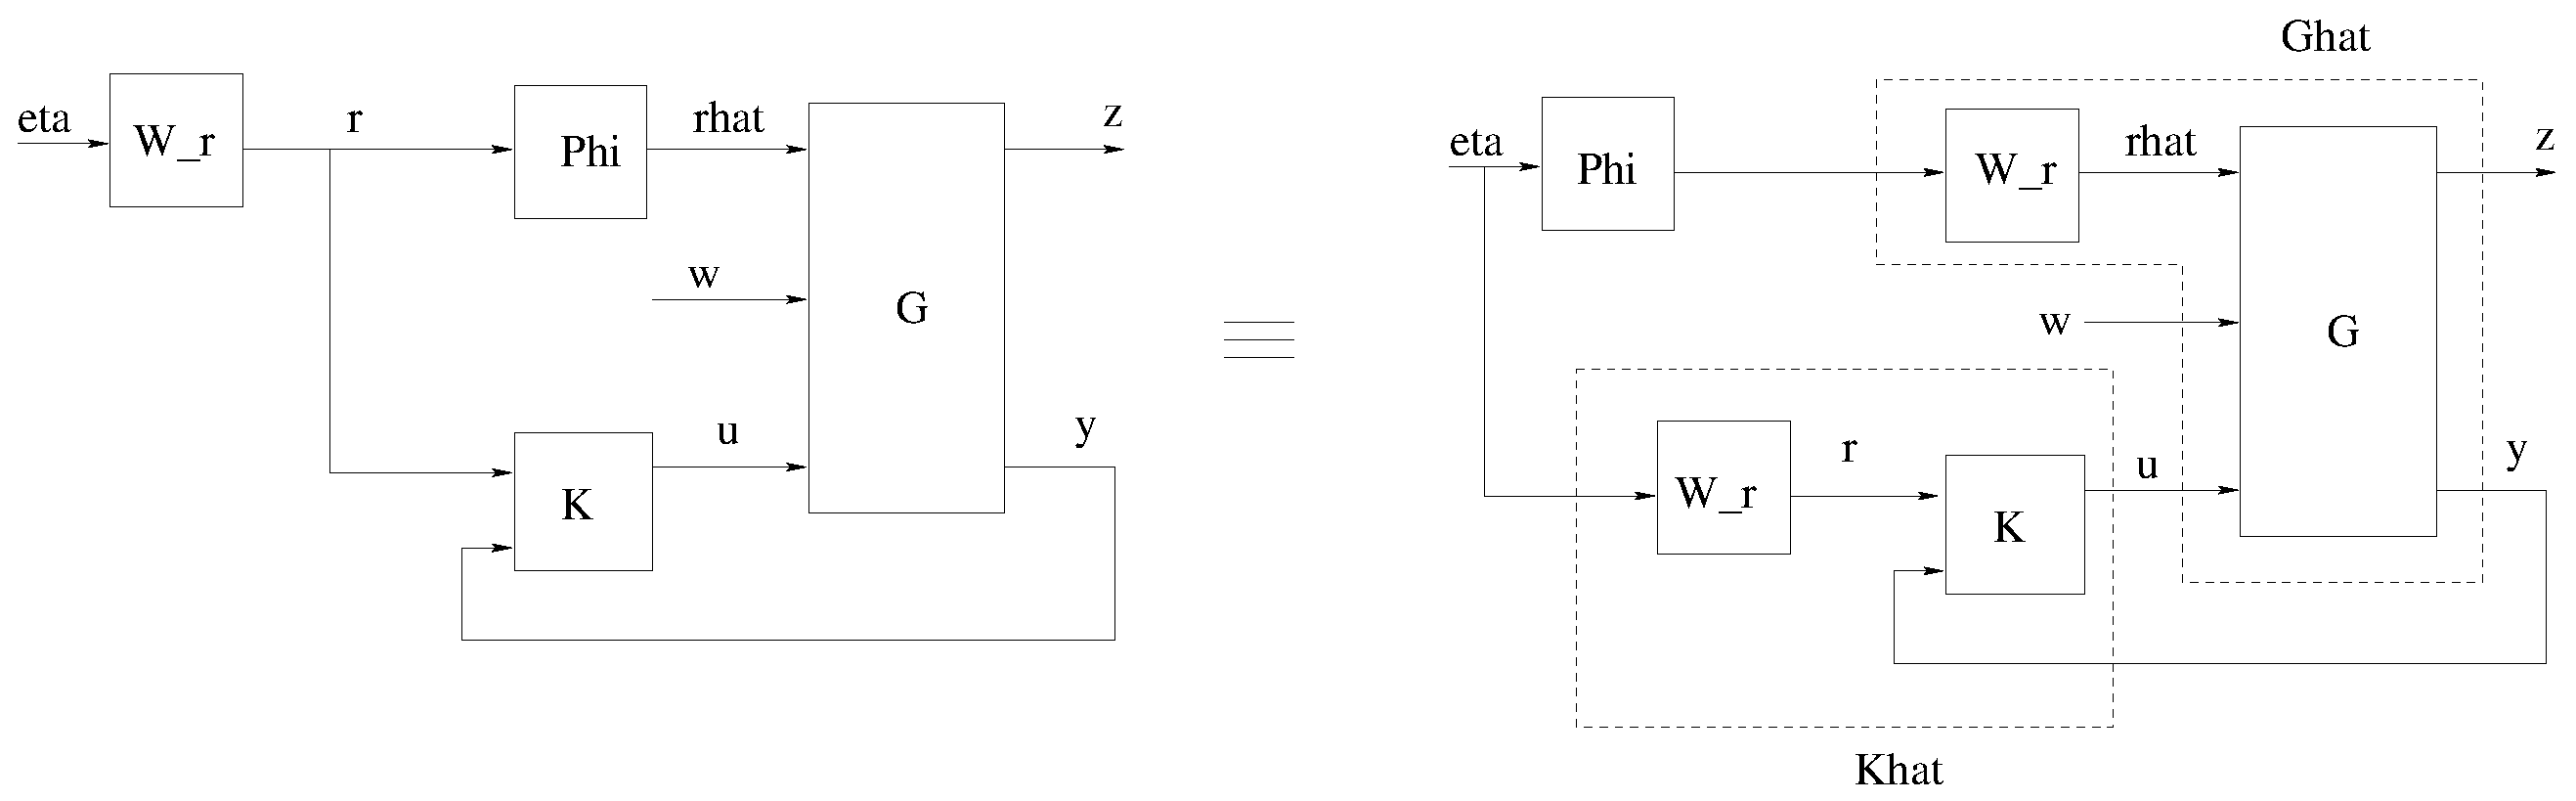
\includegraphics[width=1.4\columnwidth]{./diags/DistRejSysEquiv.eps}}
\end{center}
\caption{Two equivalent representations of the previewable disturbance rejection problem. These representations are equivalent in the sense that the transfer functions from $\eta$ and $w$ to $z$ and $y$ are identical. Recall that $\Phi=\z^{-N}I$, which commutes with $W_r$ under multiplication. \label{fig:AbsorbWr}}
\end{figure}

For the purposes of computing the minimum achievable $\htwo$-norm, we may assume $W_r=I$ without loss of generality. The transformation that enables us to make this assumption is illustrated in Figure~\ref{fig:AbsorbWr}. The design problem involving $\hat K$ and $\hat G$ is clearly a problem of the class of Figure \ref{fig:DistRejSys}, but without a pre-filter. The achievable $\htwo$-norm will be the same in either case, and in this section we will work with the simpler problem setup, where it is assumed that $W_r$ has been absorbed into $\hat G$ and $\hat K$. This transformation is not used in the preceding sections because it obscures the impact of $W_r$ on the control signal, and because we would be required to perform further manipulations in order to remove the additional controller states resulting from the extra copy of $W_r$. 

It is easy to check that the results of the previous sections carry over for $W_r=I$. All that is required is to remove the  gains associated with the states of $W_r$.

We note again that:
% 
\begin{equation}
\nrm{T_{{[r'\,\,w']'}\rightarrow z}}^2_2 =
\nrm{T_{w\rightarrow z}}^2_2+
\nrm{T_{r\rightarrow z}}^2_2. \label{proj_prop}
\end{equation}
%
As observed in Corollary~\ref{cor:minwandr}, the optimal preview controller minimises $\nrm{T_{w\rightarrow z}}_2$. Since $X_{gg}$ and $Y_g$ are the solutions to the DAREs associated with the problem of minimising $\nrm{T_{w\rightarrow z}}_2$, we may use the results in Sections \ref{subsec:stdH2FI} and \ref{subsec:stdH2OF} to write:
\als{
\gamma_{wc}^2&=\textrm{Tr}\left\{(D_{11gw}+D_{12}F_{0w})'(D_{11gw}+D_{12}F_{0w})\right.\\ &\left.\qquad+(B_{1gw}+B_{2g}F_{0w})'X_{gg}(B_{1gw}+B_{2g}F_{0w})\right\}\\
\gamma_{wf}^2&=\textrm{Tr}\left\{\bar R\left( (L_{0y}D_{21gw}-F_{0w})(L_{0y}D_{21gw}-F_{0w})'\right.\right.\\ &\left.\left.\qquad+(L_{0y}C_{2g}-F_{2g})Y_{gg}(L_{0y}C_{2g}-F_{2g})'\right) \right\}\\
\nrm{T_{w\rightarrow z}}^2_2&=\gamma_{wc}^2+\gamma_{wf}^2,
} 
which are independent of the preview length.

We now turn our attention to the evaluation of $\nrm{T_{r\rightarrow z}}_2$. Since the signal $r$ is `known' to the controller, it does not introduce an estimation error. As a result the output feedback controller achieves exactly the same transfer function $T_{r\rightarrow z}$ as the full-information controller, $K_{FI}$. Thus:
\als{
T_{r\rightarrow z}=\ssmodf{A+B_2F_2}{\ma{B_{2g}F_{0r}\\B_p}}{C_1+D_{12}F_2}{D_{12}F_{0r}}.
}
%
Note that $X$ satisfies: 
\als{(A+B_2F_2)'X(A+B_2F_2)+(C_1+D_{12}F_2)'(C_1+D_{12}F_2),}
and so using equation (\ref{eqn:2normcomp}) we may write:
\als{
\nrm{T_{r\rightarrow z}}^2_2 &=\tra{\left(D_{12}F_{0r}\right)'D_{12}F_{0r}+\ma{B_{2g}F_{0r}\\B_p}'\ma{X_{gg}&X_{gp}\\X_{gp}'&X_{pp}}\ma{B_{2g}F_{0r}\\B_p}}.
} 
\mbox{where $F_{0r}=-{\bar R}^{-1}B_{2g}'X_{gp}B_p$. The above expression may be simplified to} 
\aln{
\nrm{T_{r\rightarrow z}}^2_2&=\tra{B_p'X_{pp}B_p-F_{0r}'\bar RF_{0r}\label{eqn:gamrmedeff}}.
}
%
Our next task is to find an efficient method for computing $B_p'X_{pp}B_p$. Using the $W_r=I$ version of (\ref{eqn:Xdd}), we can write:
\als{
X_{pp}&=A_p'X_{pp}A_p+\hat Q-F_{2p}'\bar{R}F_{2p}\\
\mbox{in which} \\
\hat Q &= C_{p}'B_{1gr}'X_{gg}B_{1gr}C_{p}+A_p'X_{gp}'B_{1gr}C_{p}+C_{p}'B_{1gr}'X_{gp}A_p+C_{p}'D_{11gr}'D_{11gr}C_{p}.
}

Substituting this into itself leads to:

\als{
X_{pp}=\sum^{N-1}_{j=0}{A_p^j}'(\hat Q - F_{2p}'\bar{R}F_{2p})A_p^j.
}
%
Note that post-multiplying by $A_p^kB_p$ has the effect of selecting individual block columns of the preceding matrix, that $C_pA_p^kB_p=0 \,\, \forall k \neq N-1$, and that $A_p^N=0$. This means that:
%
\[
B_p'X_{pp}B_p=B_{1gr}'X_{gg}B_{1gr}+D_{11gr}'D_{11gr}-F_{2p0}'\bar{R}F_{2p0} - \sum_{j=0}^{N-2}S' A^j_{cg} B_{2g} {\bar R}^{-1} B_{2g}' {A^j_{cg}}' S,
\]
where $F_{2p0}$ is the left-most block column of $F_{2p}$ and is given by:
\begin{equation}
F_{2p0}=-\bar R^{-1}\left(B_{2g}'X_{gg}B_{1gr}+D_{12}'D_{11gr}\right). \label{eqn:F2p0}
\end{equation}
%
Combining this with (\ref{eqn:gamrmedeff}), and using (\ref{eqn:Xgp}), leads to 
\aln{
\nrm{T_{r\rightarrow z}}^2_2=\tra{\underbrace{B_{1gr}'X_{gg}B_{1gr}+D_{11gr}'D_{11gr}-F_{2p0}'\bar{R}F_{2p0}}_{\mbox{Zero preview}}-\underbrace{\sum_{j=0}^{N-1}S' A^j_{cg} B_{2g}{\bar R}^{-1} B_{2g}'{A^j_{cg}}'S}_{\mbox{Preview reduction}}}.
\label{eqn:H2CostSplit}}
In order to judge how much preview to use, we need to know the value of the maximum possible improvement due to preview action. Suppose the matrix $\Gamma$ satisfies:
\als{
\Gamma=A_{cg}\Gamma A_{cg}'+B_{2g}\bar R^{-1}B_{2g}'
,}
which implies that:
\als{
\Gamma=\sum_{j=0}^{\infty}A_{cg}^jB_{2g}\bar R ^{-1}B_{2g}'{A_{cg}'}^{j}
.}
Comparing this to (\ref{eqn:H2CostSplit}), it follows that the reduction in $\nrm{T_{r\rightarrow z}}_2^2$ due to preview is bounded above by 
\[
\tra{S'\Gamma S},
\]
and evaluating this limit only requires the solution of an $n_g$-dimensional Lyapunov equation (in addition to the $n_g$ dimensional DARE required to evaluate $S$). The following quantity provides a useful measure of the fraction of the maximum norm reduction that has been achieved:
\aln{\gamma_{\,_{\%,imp}}=100\times \tra{S'\Gamma S}^{-1}{\left(\sum_{j=0}^{N-1}S' A^j_{cg} B_{2g}{\bar R}^{-1} B_{2g}'{A^j_{cg}}'S\right)}.\label{eqn:gamimp}} 
%This provides a useful bound on the achievable norm reduction one might obtain using preview. 
This can be used to determine how much preview to use; for example, one might continue adding preview points until $\gamma_{\,_{\%,imp}} >99\%$.

 
\section{Computation of preview feedforward controller} 
\label{sec:Preproc}
In this section we consider the problem of designing a feedforward controller. Such a problem may arise if there is no feedback signal, or if we wish to use a preview precompensator to enhance an existing feedback controller. 

%It follows from (\ref{proj_prop}) and the fact that a feedforward controller does not alter $T_{w\rightarrow z}$, that $\nrm{T_{[w'\,\, \eta']'\rightarrow z}}_2$ is minimised by choosing the feedforward controller which minimises $\nrm{T_{\eta \rightarrow z}}_2$. 

Potentially, one could formulate a feedforward problem by removing the measurement signal $y$ from the configuration in Figure~\ref{fig:DistRejSys}. However, if we recall that 
\als{
\nrm{T_{{[\eta'\,\,w']'}\rightarrow z}}^2_2 =
\nrm{T_{w\rightarrow z}}^2_2+
\nrm{T_{\eta\rightarrow z}}^2_2,}
and that a feedforward controller does not alter $T_{w\rightarrow z}$, then it follows that $\nrm{T_{[w'\,\, \eta']'\rightarrow z}}_2$ is minimised by choosing the feedforward controller which minimises $\nrm{T_{\eta \rightarrow z}}_2$.  Given these observations, we may neglect the influence of $w$ in the design process.

\begin{figure}
\begin{center}
\stdcontrolfrags
\psfrag{rhat}{}
\psfrag{KFF}{$K_{FF}$}
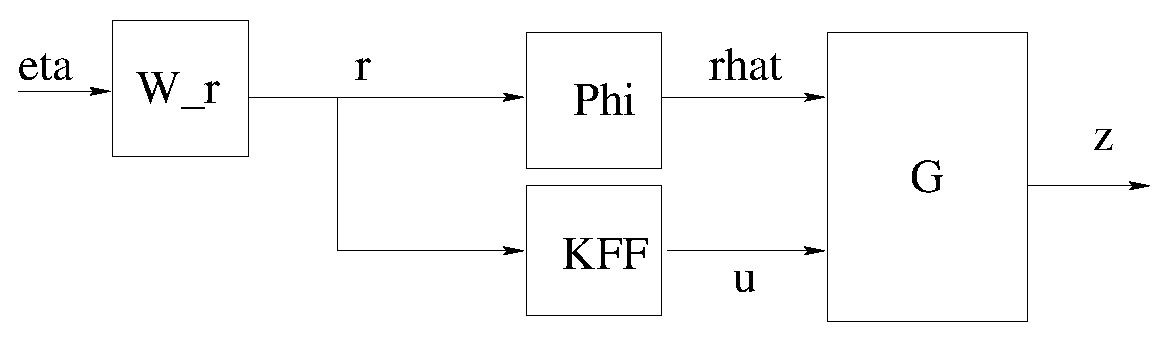
\includegraphics[width=9cm]{./diags/DistRejSysFF.eps}
\end{center}
\caption{A feedforward controller design problem. The notation follows that of Figure \ref{fig:DistRejSys}.\label{fig:DistRejSysFF}}
\end{figure}

The problem considered in this section is illustrated in Figure \ref{fig:DistRejSysFF}. Such a configuration is apparently a special case of Figure~\ref{fig:DistRejSys}, and so it is tempting to try to tackle this problem by using the above general theory with $y$ set to zero (by setting $D_{21gw}$, $D_{21gr}$, $C_{2g}$ and $D_{22g}$ to zero) and with $w$ removed. Unfortunately, such an approach does not succeed because assumption (A5) is violated. We will now derive a solution to this problem.

By modifying (\ref{eqn:P}), it follows that the appropriate generalised plant is given by:
\aln{
P_{FF}&\shorteq\ma{\arr{cc|c:c}{
A_g&B_{1gr}C_{d1}&0&B_{2g}\\
0&A_d&B_{d}&0\\\hline
C_{1g} &D_{11gr}C_{d1} &0&D_{12}\\ \hdashline
0&C_{d2}&D_r&0
}}\label{eqn:PFF}\\
&=\ssmod{A}{B_1}{B_2}{C_1}{C_2}{D_{11}}{D_{12}}{D_{21}}{0}
.}

It is easily checked that the associated full-information control is obtained by removing the gain associated with $w$, and so  $K_{FI}=\ma{F_{2g} &F_{2p}&F_{2r} & F_{0r} }$, where the gains may be computed using (\ref{eqn:F2g}) and (\ref{eqn:F2pEff})-(\ref{eqn:F0reff}). To arrive at this result one need only retrace the derivations of Section \ref{sec:H2FI}, with $B_{1gw}$ and $D_{11gw}$ set to zero.

Next, we give a result concerning the solution to the estimation DARE:
\begin{lem}
If $A_g$ is stable and $W_r$ is outer, then the version of the DARE (\ref{eqn:Y2d}) associated with (\ref{eqn:PFF}) has a stabilising solution $Y=0$.
\end{lem}
\begin{proof}
First note that if $Y=0$, then:
\als{
L_2&= -\ma{0\\B_dD_r^{-1}}\\
\bar S&= D_rD_r'
,}
from which it can be checked that $Y=0$ solves (\ref{eqn:Y2d}). This solution is stabilising because:
\als{
A+L_2C_2=\ma{A_g &B_{1gr}C_{d1}\\0&A_d-B_dD_r^{-1}C_{d2}  }
}
is stable since $A_g$ is stable and $W_r$ is outer (see (\ref{eqn:AdBdDrCd2})).
\end{proof}
If we also note that:
\als{L_0&= F_{0r}D_r^{-1},}
with $F_{0r}$ defined in (\ref{eqn:F0reff}),
then we can use (\ref{eqn:H2OptK}) to obtain the following $\htwo$-optimal controller:
\als{
K_{FF}& \shorteq \ma{\arr{c|c}{A_K&B_K\\\hline C_K&D_K}}\\
A_K&=\ma{A_g+B_{2g}F_{2g}&B_{1gr}C_p+B_{2g}F_{2p}&B_{2g}F_{2r}-B_{2g}F_{0r}D_r^{-1}C_r\\
0&A_p&0\\
0&0&A_r-B_rD_r^{-1}C_r}\\
B_K&=\ma{B_{2g}F_{0r}D_r^{-1}\\
	B_p\\
	B_rD_r^{-1}}\\
C_K&=\ma{F_{2g}&F_{2p}&F_{2r}-F_{0r}D_r^{-1}C_r}\\
D_K&=F_{0r}D_r^{-1}
,}
%
which has the low order representation:
\als{
\bar K_{FF} \shorteq \ma{\arr{cc|cc}{
A_g+B_{2g}F_{2g}&B_{2g}F_{2r}-B_{2g}F_{0r}D_r^{-1}C_r  & B_{1gr}C_p+B_{2g}F_{2p} & B_{2g}F_{0r}D_r^{-1}\\
0 & A_r-B_rD_r^{-1}C_r & 0 & B_rD_r^{-1}\\\hline
F_{2g} & F_{2r}-F_{0r}D_r^{-1}C_r & F_{2p} & F_{0r}D_r^{-1}
}}}
%
such that the optimal control is given by:
\als{
u^*&=\bar K_{FF} \bar r
}
in which
\als{
\bar r(k)&=\ma{r(k-N)\\\vdots\\r(k)}.
}


\section{Summary of Results} 
\label{sec:H2PrevSum}
Our purpose here is to provide a summary of the major features of $\htwo$ preview controllers, which will hopefully be of assistance to control system designers. While some of these results are known within the control systems community, they are spread over many publications spanning three decades. 
\subsection{Generic Controller features} \label{generic:features}
\begin{description}
\item[Riccati Equation Solutions.] Synthesizing the output-feedback controller requires the solution of a full-information Riccati equation and a Kalman filtering equation \cite{LimebeerGreen,ZDG}. Although these equations appear to be of high order, the full-information control problem only requires the solution of the $n_g$-dimensional Ricatti equation (\ref{eqn:Xgg}), while the estimation problem requires the solution of the $n_g$-dimensional Riccati equation (\ref{eqn:Y2g}). The bulk of the full-information Riccati equation can be evaluated using the linear equations (\ref{eqn:Xgd}) and (\ref{eqn:Xdd}). The DARE (\ref{eqn:Xgg}) is precisely that which would be obtained if one were to search for a full information controller which minimised $\nrm{T_{w\rightarrow z}}$.

It is important to note that $F_{2g}$ and $\bar R$ are not functions of $X_{gd}$ or $X_{dd}$, and so (\ref{eqn:Xgg}) may be solved independently of (\ref{eqn:Xgd}) and (\ref{eqn:Xdd}). However, (\ref{eqn:Xgd}) depends on the solution of (\ref{eqn:Xgg}), and (\ref{eqn:Xdd}) depends on both (\ref{eqn:Xgg}) and (\ref{eqn:Xgd}). Lemma~\ref{lem:SylvRecurs} provides a fast algorithm for solving (\ref{eqn:Xgd}).
\item[Full-information control structure.] The full-information control signal has the form
\als{
u(k)^*=\hat u(k)+\sum_{j=0}^{N-1}{F_{2p,j}r(k-N+j)},
}
in which $\hat u(k)$ is a linear function of the states of $G$ and $W_r$, and of the signals $\eta$ and $w$; the $F_{2p,j}$'s are sometimes referred to as the `preview gains'. Further insight into the structure and role of the control signal components can be found in Remarks~\ref{rem:PrevGainInterp}, \ref{rem:SmallPrevGain} and \ref{rem:FIminwandr}.
\item[The preview gains decay to zero as $N \rightarrow \infty$.] It was first noted in \cite{Tomizuka_1975_OptDiscretePreview} that the magnitude of the preview gains approaches zero as $N$ approaches infinity; this follows from equation (\ref{eqn:F2pEff}) and $\lim_{N \rightarrow \infty} A^N_{cg} = 0$. As a consequence, far-distant preview information is relatively less important and the optimal infinite preview controller can be approximated  to arbitrary accuracy using a finite preview length.
\item[The controller has FIR (preview) and IIR components.]
Discrete-time preview controllers are composed of a high-order Finite Impulse Response (FIR) preview component, and low-order {IIR} components. This structure is illustrated in Figure~\ref{fig:PrevContStruct}, and is also highlighted in the continuous-time case in \cite{Moelja_2006_H2PreviewMultiple}. A proof is provided for the discrete-time case in Section \ref{sec:H2OF}. If the controller is written in observer form, then the states of the FIR preview block and the order $n_r$ IIR block are (perfect) reconstructions of the states of $\Phi$ and $W_r$ respectively. The state of the order $n_g$ IIR block is an estimate for the state of $G$.
\item[The controller is essentially low-order.] 
A discrete-time FIR transfer function can be realised using a shift-register to update the state, and a gain array to compute the output. This representation leads to the low-order controller representation in Figure~\ref{fig:PrevContStructxp}, where $\bar{K}$ is given by (\ref{low_order_K}). 
{
\stdcontrolfrags
\psfrag{Kbar}{$\bar K$}
\psfrag{Kr}{$K_r$}
\psfrag{r}{$r(k)$}
\psfrag{y}{$y(k)$}
\psfrag{u}{$u(k)$}
\psfrag{xpr}{$\ma{r(k-N)\\\vdots\\r(k)}$}
\begin{figure}
\begin{center}
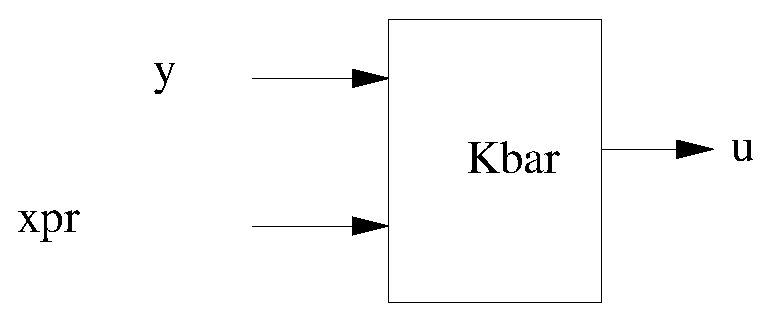
\includegraphics[width=0.42\columnwidth]{./diags/PrevContStructxpKbar.eps}
\caption{\label{fig:PrevContStructxp} The structure of the $\htwo$-optimal discrete-time preview controller. The signal $u(k)$ is the control, the measurement is $y(k)$, and $r(k)$ is the future-most value of the previewable disturbance.}
\end{center}
\end{figure}}\item[The optimal control is independent of $W_r$ for large $N$]
This phenomenon was first noticed in \cite{Tomizuka_1975_OptDiscretePreview}, with a proof provided in Section \ref{sec:H2FI}. It is instructive to consider the influence of $W_r$ from a stochastic perspective. Since $\eta$ is assumed to be a realisation of a white-noise process, then a dynamic $W_r$ provides statistical information on future values of $r$. If, for example, $W_r$ is low-pass, the $r(k)$'s become correlated and hence $W_r$ introduces `statistical preview' beyond the preview horizon. We would therefore expect $W_r$ to reduce the need for preview, and also that its influence on the control would decline as $N$ tends to infinity.
\item[The optimal $\nrm{T_{w\rightarrow z}}_2$ is independent of $W_r$.]
In contrast with the $\hinf$ case \cite{Hazell_2007_DiscreteHinfPreview}, there is no conflict between the rejection of $w$ and the rejection of $\eta$; a proof of this is provided in Section \ref{sec:H2OF}.
\item[Noisy preview signals require a high-order controller.]
One might consider an uncertain preview problem, where the controller has access only to a noise-corrupted version of the previewed signal. 
In this scenario, the states of $\Phi$ are not known, and must be estimated. The preview provides benefit both by reducing the Full Information control cost, and by reducing the estimation cost. Estimating the states of $\Phi$ is a type of fixed-lag smoothing problem. Low-order implementations of fixed-lag smoothers are given in \cite{Anderson_1979_OptimalFiltering}, but these implementations are not usable here, because of the need for an estimate of all of the states of $\Phi$, rather than just the output of $\Phi$. The resulting controller is thus of the same order as the augmented plant. A controller for this problem may be synthesised by direct application of the results in Section \ref{subsec:stdH2OF}.
\end{description}
\subsection{Design Insights}
This section provides a number of `rules of thumb' that the authors have found useful. For the purposes of illustration, we will consider the full-information preview tracking problem described in Figure~\ref{fig:PrevTrackSysFI}, where $G$ is given by:
\begin{eqnarray}
\hat G&=&\frac{1.26 \times 10^{-8} (\z+1)^3}{
		(\z-1) (\z^2  - 1.998\z + 0.998)} \nonumber \\
G&=&\ma{\hat G\\1}. \label{example}
\end{eqnarray}
\begin{figure}
\begin{center}
\psfrag{W_e}{$W_e$}
\psfrag{z1}{$z_1$}
\psfrag{z2}{$z_2$}
\psfrag{W_r}{$W_r$}
\psfrag{u}{$u$}
\psfrag{r}{$r$}
\psfrag{G}{$G$}
\psfrag{zg}{$z_g$}
\psfrag{Phi}{$\Phi$}
\psfrag{W_r}{$W_r$}
\psfrag{eta}{$\eta$}
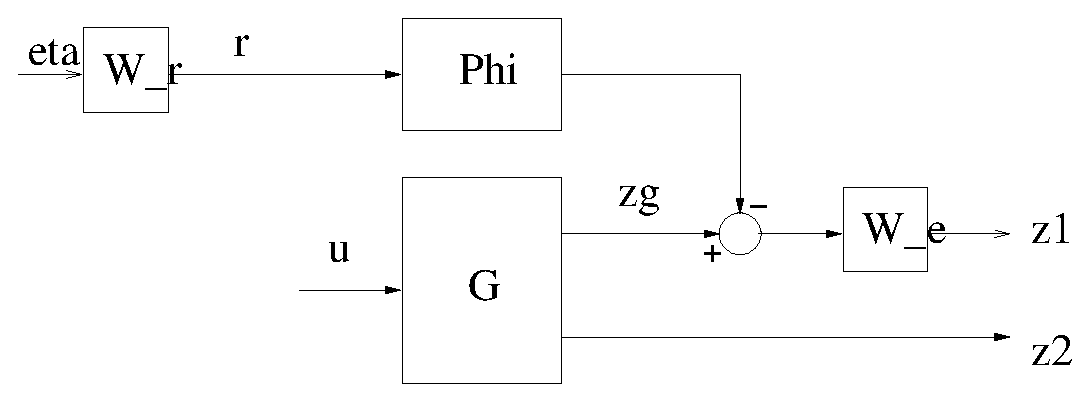
\includegraphics[width=0.75\columnwidth]{./diags/PrevTrackSysFI.eps}
\end{center}
\caption{A simple preview tracking problem. The feedback signal is derived from the states of $G$, $W_r$, $W_e$ and $\Phi$, together with $\eta$. The signal $u$ is the control, $r$ is the previewed reference, and $z=\left[z_1'\,\,z_2'\right]'$ is the output to be minimized. \label{fig:PrevTrackSysFI}}
\end{figure}
The discrete transfer function $\hat G$ was obtained by discretising
\als{       \frac{101}{s (s^2 + 2s + 101)},}
using a sample time of 0.001 seconds.
We search for a $K$ which minimises $\nrm{T_{\eta\rightarrow z}}_{2,\infty}$, or equivalently, the $K$ which minimises:
\aln{
\nrm{\ma{W_eW_rT_{r\rightarrow e}\\W_rT_{r\rightarrow u}}}_{2,\infty} \label{eqn:DesInsightCL}
.}
Clearly this represents a tracking problem in which minimisation of tracking errors must be balanced against  excessive control requirements. The transfer functions $W_r$ and $W_e$ may be chosen to reflect, respectively, the expected frequency content of $r$, and the importance of achieving good tracking at a given frequency. We will now use this example to illustrate some general properties of $\htwo$ preview tracking controllers.

\begin{description}
\item[Preview improves steady-state tracking.] 
Figure~\ref{fig:BetterSSWithIncN} illustrates the `non-responsiveness' of the closed-loop system in the case of no reference weight, and a low preview horizon. In the limiting case, where there is zero preview and no reference weighting, the controller does not have any information about the value of the reference at the next time step, and so it cannot make a decision about the direction in which to send the plant. Therefore, the tracking error cost cannot be reduced, and so the optimal controller can only minimise the control cost, leading to a choice of $u=0$.

Alternatively, as $N\rightarrow \infty$, then the steady state error tends towards zero (in the absence of disturbances or modelling errors). 
\begin{figure}
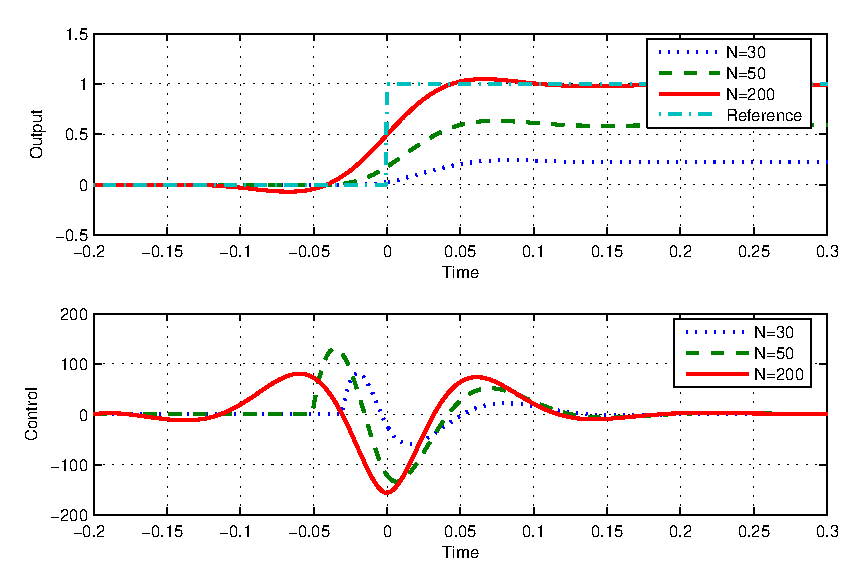
\includegraphics[width=\columnwidth]{./diags/BetterSSwithIncN.eps}
\caption{Closed-loop response of the system described in (\ref{example}) and Figure~\ref{fig:PrevTrackSysFI} with $W_r=1$ and $W_e=1000$.
The plotted output is the signal $z_g$ in Figure~\ref{fig:PrevTrackSysFI}, and shows the relative non-responsiveness of the low-preview-horizon system.
\label{fig:BetterSSWithIncN}}
\end{figure}
%Changes merged to here
\item[Reference weighting introduces stochastic preview.] 
The responses illustrated in Figure \ref{fig:BetterSSWithIncN} are unsatisfactory for preview horizons of less than $N=200$. When short preview horizons are mandated, a low-pass $W_r$ improves low frequency tracking by biasing the controller optimisation towards lower frequencies. It is worth noting, however, that care should be taken in choosing $W_r$.
If, for example, $W_r$ rolls off too quickly, the closed-loop will be poorly tuned for step inputs and can have an oscillatory response, and/or high-amplitude controls. This is because a low-pass $W_r$ has the dual effect of penalising low frequency tracking errors, and also reducing the penalty on high frequency controls -- see (\ref{eqn:DesInsightCL}).
The effect of a low-pass $W_r$ is illustrated in Figure~\ref{fig:WrWithIncreasingPreview}.
\begin{figure}
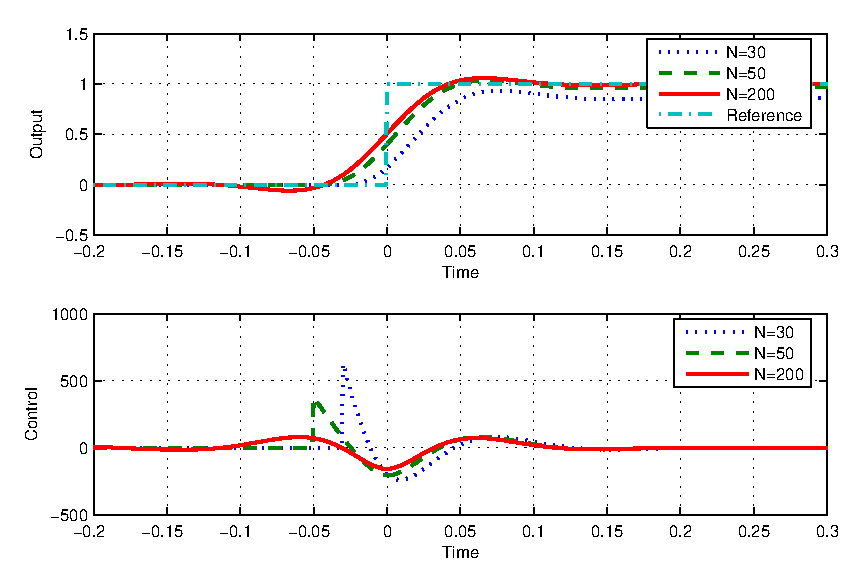
\includegraphics[width=\columnwidth]{./diags/WrWithIncreasingPreview.eps}
\caption{Closed-loop response of the system described in (\ref{example}) and Figure~\ref{fig:PrevTrackSysFI}; the reference weight is given by $W_r=\z/(\z-0.99)$, with $W_e=1000$. The improved step response (of $z_g$) for short preview horizons is clearly visible. Note the high-amplitude control in the $N=30$ case. \label{fig:WrWithIncreasingPreview}}
\end{figure}
\item[Tracking-error filtering.]
Consider the Full Information controller synthesis problem illustrated in Figure~\ref{fig:PrevTrackSysFI} and let $W_e$ be a dynamic
tracking-error filter. A low-pass weight on the tracking error improves the low-frequency tracking performance, without needing to change the assumed frequency content of the reference signal (i.e. without changing $W_r$). Note that a step change in the reference does not lead to a `spike' in the control signal -- see Figure \ref{fig:ReducingControlWithIncreasingN}. 
\item[Improving the low-frequency tracking behaviour.]
It appears that there are three alternative ways of improving the low-frequency tracking behaviour, which could be used alone or in combination: (A) use a long preview horizon; (B) add a low-pass reference filter, and (C) introduce a low-pass tracking-error filter. These alternatives are illustrated in Figure~\ref{fig:CompWzWrNormForSimilarResp}. In order to achieve a fair comparison, $W_e$ was scaled so that the resulting closed loops achieved approximately similar rise times. The tracking-error filter achieves good steady-state performance without excessive control, or large control spikes.
However, the introduction of a tracking-error filter tends to introduce additional phase lag, which can have a deleterious effect on the loop's robust stability. In contrast, the feedback part of the controller is independent of $W_r$, which means that a reference filter can be used without jeopardising stability.  
\begin{figure}
\begin{center}
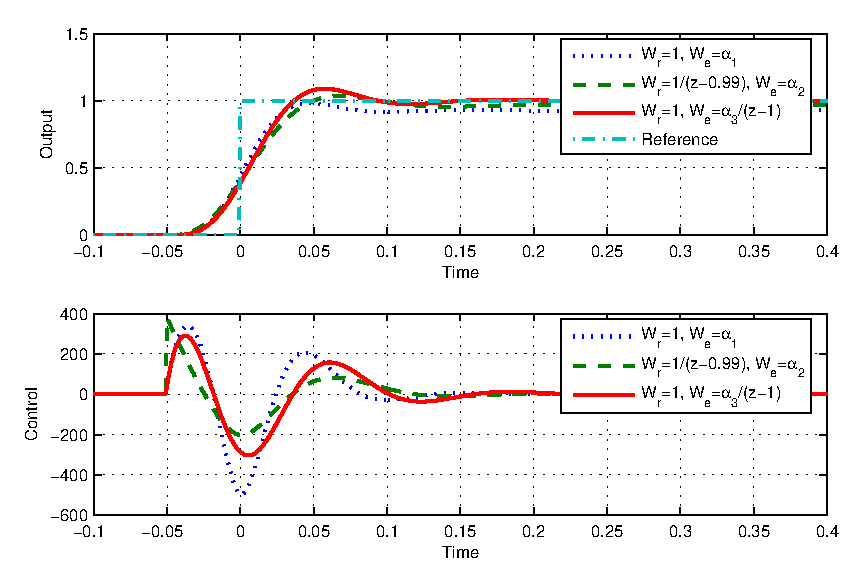
\includegraphics[width=\columnwidth]{./diags/CompWzWrNormForSimilarResp.eps}
\end{center}	
\caption{Closed-loop response of the example system described in (\ref{example}) and Figure~\ref{fig:PrevTrackSysFI}. The preview horizon is fixed at $N=50$ and $\alpha_i$ is used to achieve similar closed-loop rise times. While the closed-loop responses ($z_g$) are similar, the control signals are quite different; especially near the beginning of the preview horizon. \label{fig:CompWzWrNormForSimilarResp}}
\end{figure}
\item[Preview reduces the peak control magnitude.] 
Figure~\ref{fig:ReducingControlWithIncreasingN} illustrates the influence of preview on the control magnitude. In this example, the output response is not strongly influenced by changes in the preview horizon, but the peak control magnitude reduces substantially as the preview horizon increases. This effect can be very useful in application in which control ceilings are a limiting factor, and one wishes to maintain a short rise time.
\begin{figure}
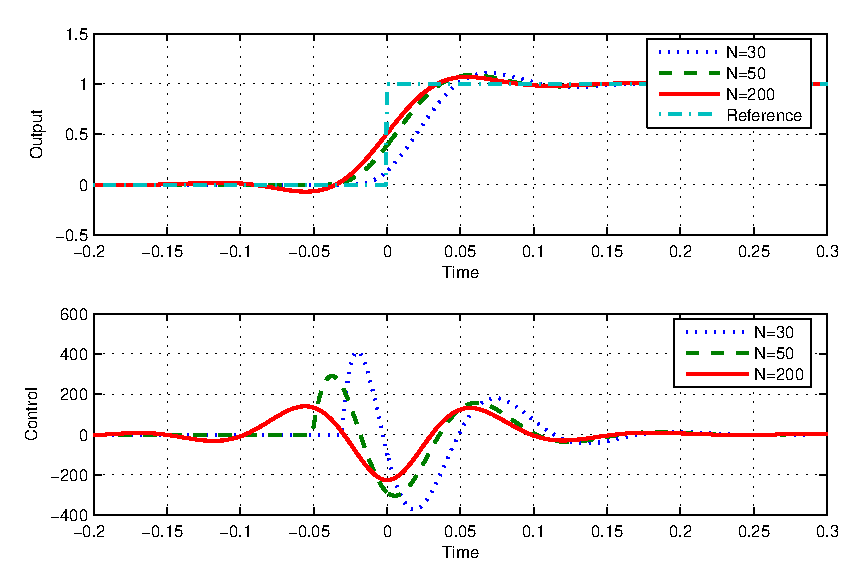
\includegraphics[width=\columnwidth]{./diags/ReducingControlWithIncreasingN.eps}
\caption{Closed-loop response of the example system described in (\ref{example}) and Figure~\ref{fig:PrevTrackSysFI}; the weighting functions are $W_r=1$ and $W_e=100/(1-\z)$. The plotted output is the signal $z_g$ in Figure~\ref{fig:PrevTrackSysFI}, and is relatively insensitive to the preview horizon. The control signal becomes `spread out', and lower in amplitude, as the preview horizon is increased. \label{fig:ReducingControlWithIncreasingN}}
\end{figure}
\item[Preview only improves low frequency tracking performance.] For a low-pass plant, high frequency tracking performance is limited by the prohibitive amplitude of the control action. This is a fundamental feature of the plant and cannot be changed by anticipative action. This effect is illustrated in Figure~\ref{fig:sigmah2}, where preview improves the low-frequency performance by reducing the magnitude of both the tracking error and the control signal. %The price for this improvement appears to be larger control action at higher frequencies
\begin{figure}
\subfloat[Unweighted plant]{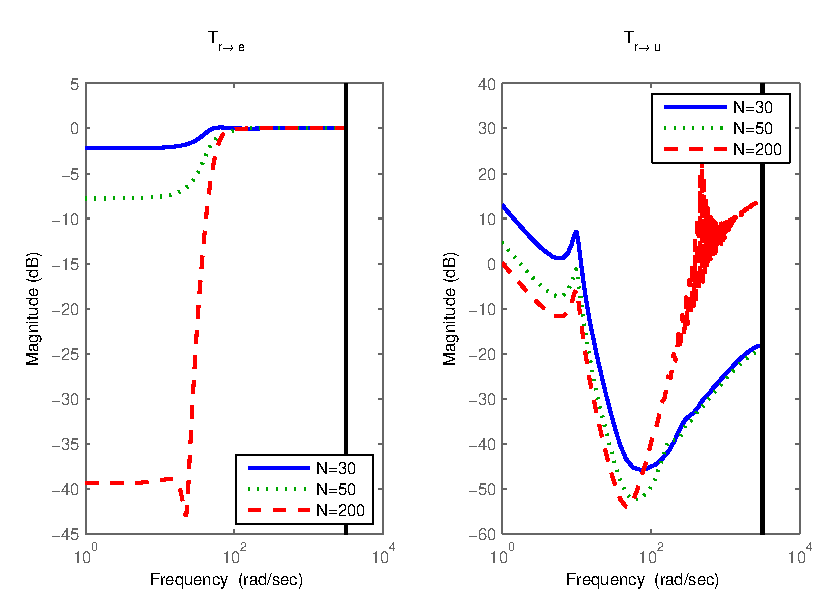
\includegraphics[width=\columnwidth]{./diags/UnweightedSigmaH2.eps}}

\subfloat[$W_e=\frac{1}{\z-1}$]{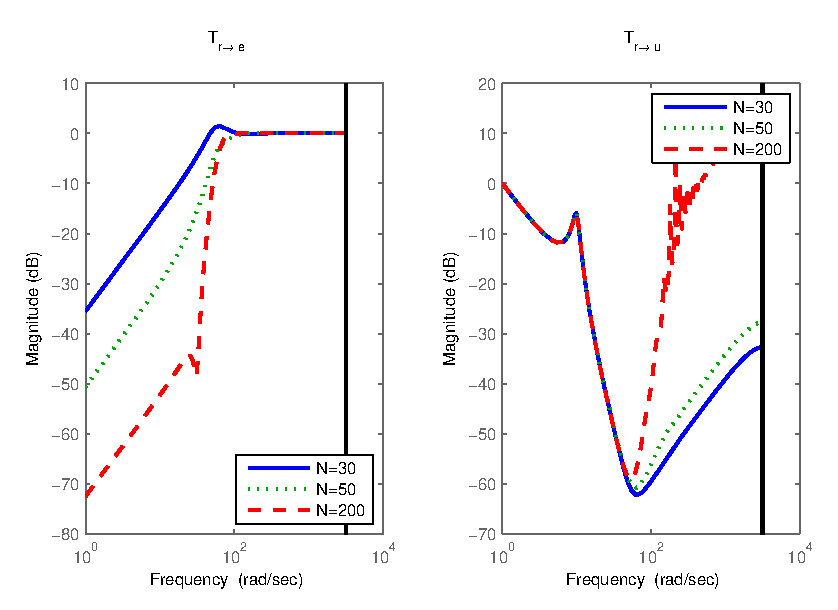
\includegraphics[width=\columnwidth]{./diags/WeightedSigmaH2.eps}}
\caption{Bode plots of the closed-loop transfer functions $T_{r\rightarrow e}$ and $T_{r\rightarrow u}$ which result from application of the $\hinf$-optimal controls.\label{fig:sigmah2} The unweighted plant is considered in (a), and a low-pass $W_e$ is employed in (b).}
\end{figure}
\item[Integral action with output feedback.]
An output-feedback tracking controller with integral action is described by Figure \ref{fig:TrackSysIntegDesign}, which also serves to
illustrate the complexity of problems that may be tackled  using the framework in Figure 1. Note that the integrated error signal must be included in the measurements in order to ensure that the integrator state is detectable. 

Tuning the relative magnitudes of $W_{e1}$ and $W_{e2}$ is akin to adjusting the gains in a PI controller. %The ability to adjust the integral gain is useful, because too much integral action can be detrimental to stability and/or the transient response. 
In fact a `derivative' signal could also be added, thus completing the PID analogy and facilitating tuning of the preview controller. 

Previously, the addition of integral action has been approached in an {LQG} setting through the use of the differentiated control signal in the cost function \citep[e.g. ][]{Tomizuka_1979_IntegralPreviewFI,Katayama_1987_PreviewAndIntegral,Tomi_1980_FFPrev}. Such an approach does not allow one to adjust the strength of the integral action, which is likely to lead to difficulty in satisfying stability/performance requirements. 


\begin{figure}
\begin{center}
\stdcontrolfrags
\psfrag{W_e1}{$W_{e1}$}
\psfrag{W_e2}{$W_{e2}$}
\psfrag{W_n}{$W_{n}$}
\psfrag{z1}{$z_1$}
\psfrag{z2}{$z_2$}
\psfrag{z3}{$z_3$}
\psfrag{y1}{$y_1$}
\psfrag{y2}{$y_2$}
\psfrag{I1/(z-1)}{$I\frac{1}{\z-1}$}
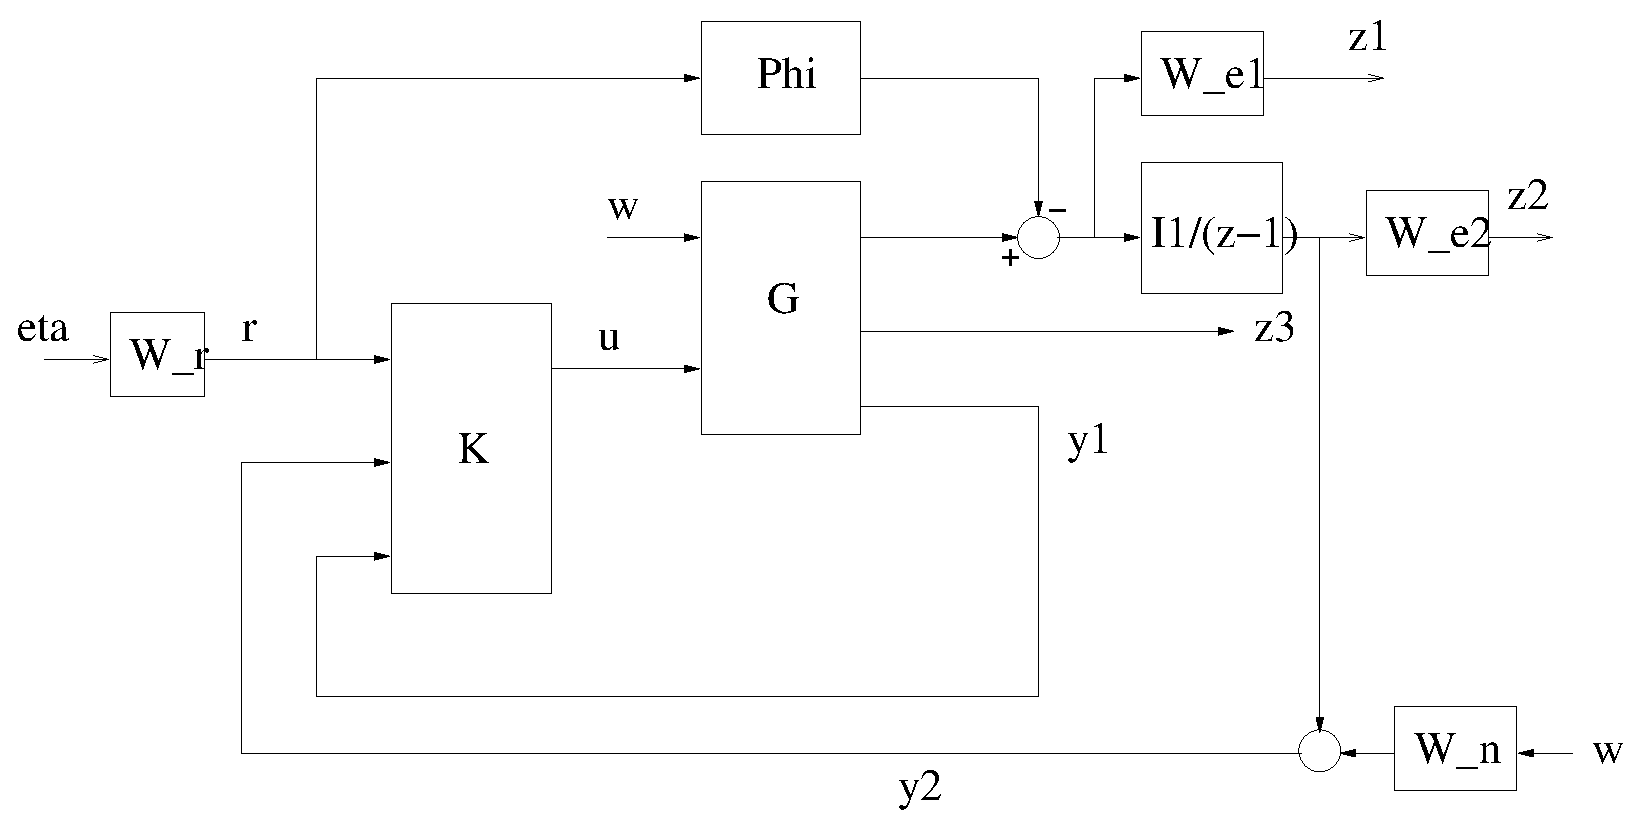
\includegraphics[width=12cm]{./diags/TrackSysInteg.eps}
\end{center}
\caption{Preview tracking with integral action. The signal $z=\left[z_1'\,\,z_2'\,\,z_3'\right]'$ is the output of the closed-loop transfer function
whose 2-norm is to be minimised; $y=\left[y_1'\,\,y_2'\right]'$ is the measurement signal. The transfer functions $W_{e1}$, $W_{e2}$ and $W_n$ are shaping filters. Other notation follows that of Figure \ref{fig:DistRejSys}. \label{fig:TrackSysIntegDesign}}
\end{figure}

\end{description}
 
\section{Concluding remarks}
\label{sec:Conclusions}
\textit{This needs re-writing to emphasise contribution. The statement that "The purpose of the present work
is to embed a class of preview control problems in a generalized regulator
configuration" is quite misleading I think. This is purely a means to an end, not the end in itself. }

\textit{Also need to reference case studies in thesis}

Preview control has been studied for over three decades and many theoretical results can be found in the technical literature. Preview control has also been employed in a variety of contempory applications in mechanical engineering. These include active automotive suspension control \cite{Roh_1999_Stoc_Opt_Prev,Marzbanrad_2004_SuspPrev}, helicopter flight control \cite{Paulino_2006_PreviewRotorcraftAffine}, 
and driver steering control \cite{Cole_2006_PredictiveAndPreviewSteeringControl}. The purpose of the present work is to embed a class of preview control problems in a generalized regulator configuration \cite{LimebeerGreen,ZDG}. The open-loop system is controlled by a two-degree-of-freedom controller, which optimizes the system response to a combination of previewable and non-previewable exogenous inputs. Efficient algorithms have been presented for solving the two standard LQG Riccati equations, as well as computing the perfect information controller gains. The associated state estimator is low order with degree $n_g+n_r$. A detailed analysis of the achievable $\htwo$-norm cost reduction due to preview is also presented. The paper concludes with a summary of the main features of $\htwo$ preview control as well as some useful design insights.





\section{Acknowledgement}  \noindent
This work was supported by a Portfolio Partnership held with the British Engineering and Physical Sciences Research Council (EPSRC), and also the Flapless Air Vehicle Integrated Industrial Research programme funded by BAe Systems and the EPSRC.

\bibliographystyle{plain}
\bibliography{./Main}

\end{document}